\documentclass[12pt]{article}
    \title{\textbf{Controllo automatico orientamento specchi forno solare}}
    \author{Scar. Francesco}
    \date{}
    \addtolength{\topmargin}{-2cm}
    \addtolength{\textheight}{3cm}
    \renewcommand{\contentsname}{Contenuti}
    \renewcommand{\figurename}{Fig.}
    
    \setlength\parindent{0pt}
    
    \newenvironment{changemargin}[2]{%
    \begin{list}{}{%
    \setlength{\topsep}{0pt}%
    \setlength{\leftmargin}{#1}%
    \setlength{\rightmargin}{#2}%
    \setlength{\listparindent}{\parindent}%
    \setlength{\itemindent}{\parindent}%
    \setlength{\parsep}{\parskip}%
    }%
    \item[]}{\end{list}}
    \long\def\/*#1*/{}          % Multiline comments https://tex.stackexchange.com/questions/87303/multi-line-block-comments-in-latex
    \usepackage{pdfpages}
    \usepackage{listings}
    \usepackage[utf8]{inputenc}
    \usepackage[T1]{fontenc}
    \usepackage{textcomp}
    \usepackage{gensymb}
    \usepackage{typearea}
    \usepackage[utf8]{inputenc}
    \usepackage[T1]{fontenc}
    \usepackage{color}
    \usepackage{mwe}
    \usepackage{listings}    
    \usepackage{etoolbox}
    \usepackage{amsmath}
    \usepackage{graphicx}
    \usepackage[hidelinks]{hyperref}
    \usepackage[hang,flushmargin]{footmisc}
    \usepackage{setspace}
    \usepackage[bottom=2.5cm]{geometry}
    
    \renewcommand{\lstlistingname}{Codice}
%    \renewcommand{\baselinestretch}{1.35}

    \definecolor{arduino_orange}{RGB}{206, 83, 1}
    \definecolor{arduino_green}{RGB}{89, 102, 6}
    \definecolor{arduino_blue}{RGB}{0, 150, 155}
    \definecolor{arduino_gray}{RGB}{170, 170, 170}
    


    \lstset{
      language = Octave,
      backgroundcolor=\color{white},   
      basicstyle=\footnotesize\ttfamily,       
      breakatwhitespace=false,         
      breaklines=true,                 
      captionpos=b,                   
      commentstyle=\color{arduino_gray},
%      deletekeywords={...},
      extendedchars=true,              
      frame=single,                    
      keepspaces=true,                 
      keywordstyle=[1]\color{arduino_orange},
      keywordstyle=[2]\color{arduino_green},
      keywordstyle=[3]\color{arduino_blue},
      %morekeywords={*,...},            
      numbers=left,
      numbersep=5pt,                   
      numberstyle=\footnotesize\color{gray}, 
      rulecolor=\color{black},         
      rulesepcolor=\color{blue},
      showspaces=false,                
      showstringspaces=false,
      showtabs=false,
      stepnumber=1,
      stringstyle=\color{orange},
      tabsize=2,                       
      title=\lstname,
%      emphstyle=\bfseries\color{blue}%  style for emph={} 
    } 

    %% language specific settings:
    \lstdefinestyle{Arduino}{%
        language = Octave,
        keywords=[1]{digitalRead, digitalWrite, micros, millis, delay, delayMicroseconds, pinMode, pow, sqrt, abs},
        keywords=[2]{if, else, while, for, do, return},%                 define keywords
        keywords=[3]{HIGH, OUTPUT, LOW, INPUT, true, false, void, int, long, unsigned, float, bool, char, uint8_t, uint18_t, int8_t, uint16_t},
        morecomment=[l]{//},%             treat // as comments
        morecomment=[s]{/*}{*/},%         define /* ... */ comments
    }

    \newtoggle{InString}{}% Keep track of if we are within a string
    \togglefalse{InString}% Assume not initally in string


\begin{document}


\maketitle

\setstretch{1}
\tableofcontents{}

\setstretch{1.3}

\newpage


\section{Introduzione}
    \subsection{Descrizione}
    Si desidera realizzare un sistema di controllo automatico dell'orientamento e inclinazione degli specchi di un forno solare per garantire la massima efficienza al variare della posizione relativa del sole nell'arco della giornata.
    Si desidera inoltre monitorare la temperatura e lo stato di funzionamento generale del sistema mediante un'interfaccia web che permetta di visualizzare un grafico in tempo reale dell'andamento della temperatura.


    \subsection{Struttura generale}
    Il sistema è composto da un contenitore di materiale isolante con la faccia superiore di vetro trasparente che permette alla luce solare di irradiare energia all'interno. La luce solare viene inoltre riflessa da due specchi posti ai lati opposti della faccia superiore (in particolare il lato superiore e quello inferiore).\\
    L'intera struttura è solidale ad una base girevole, controllata da un motore, che permette la regolazione dell'azimut, mentre l'inclinazione di ogni specchio è regolata singolarmente in funzione dell'elevazione del sole.
    
    \begin{figure}[h]
    \centering
        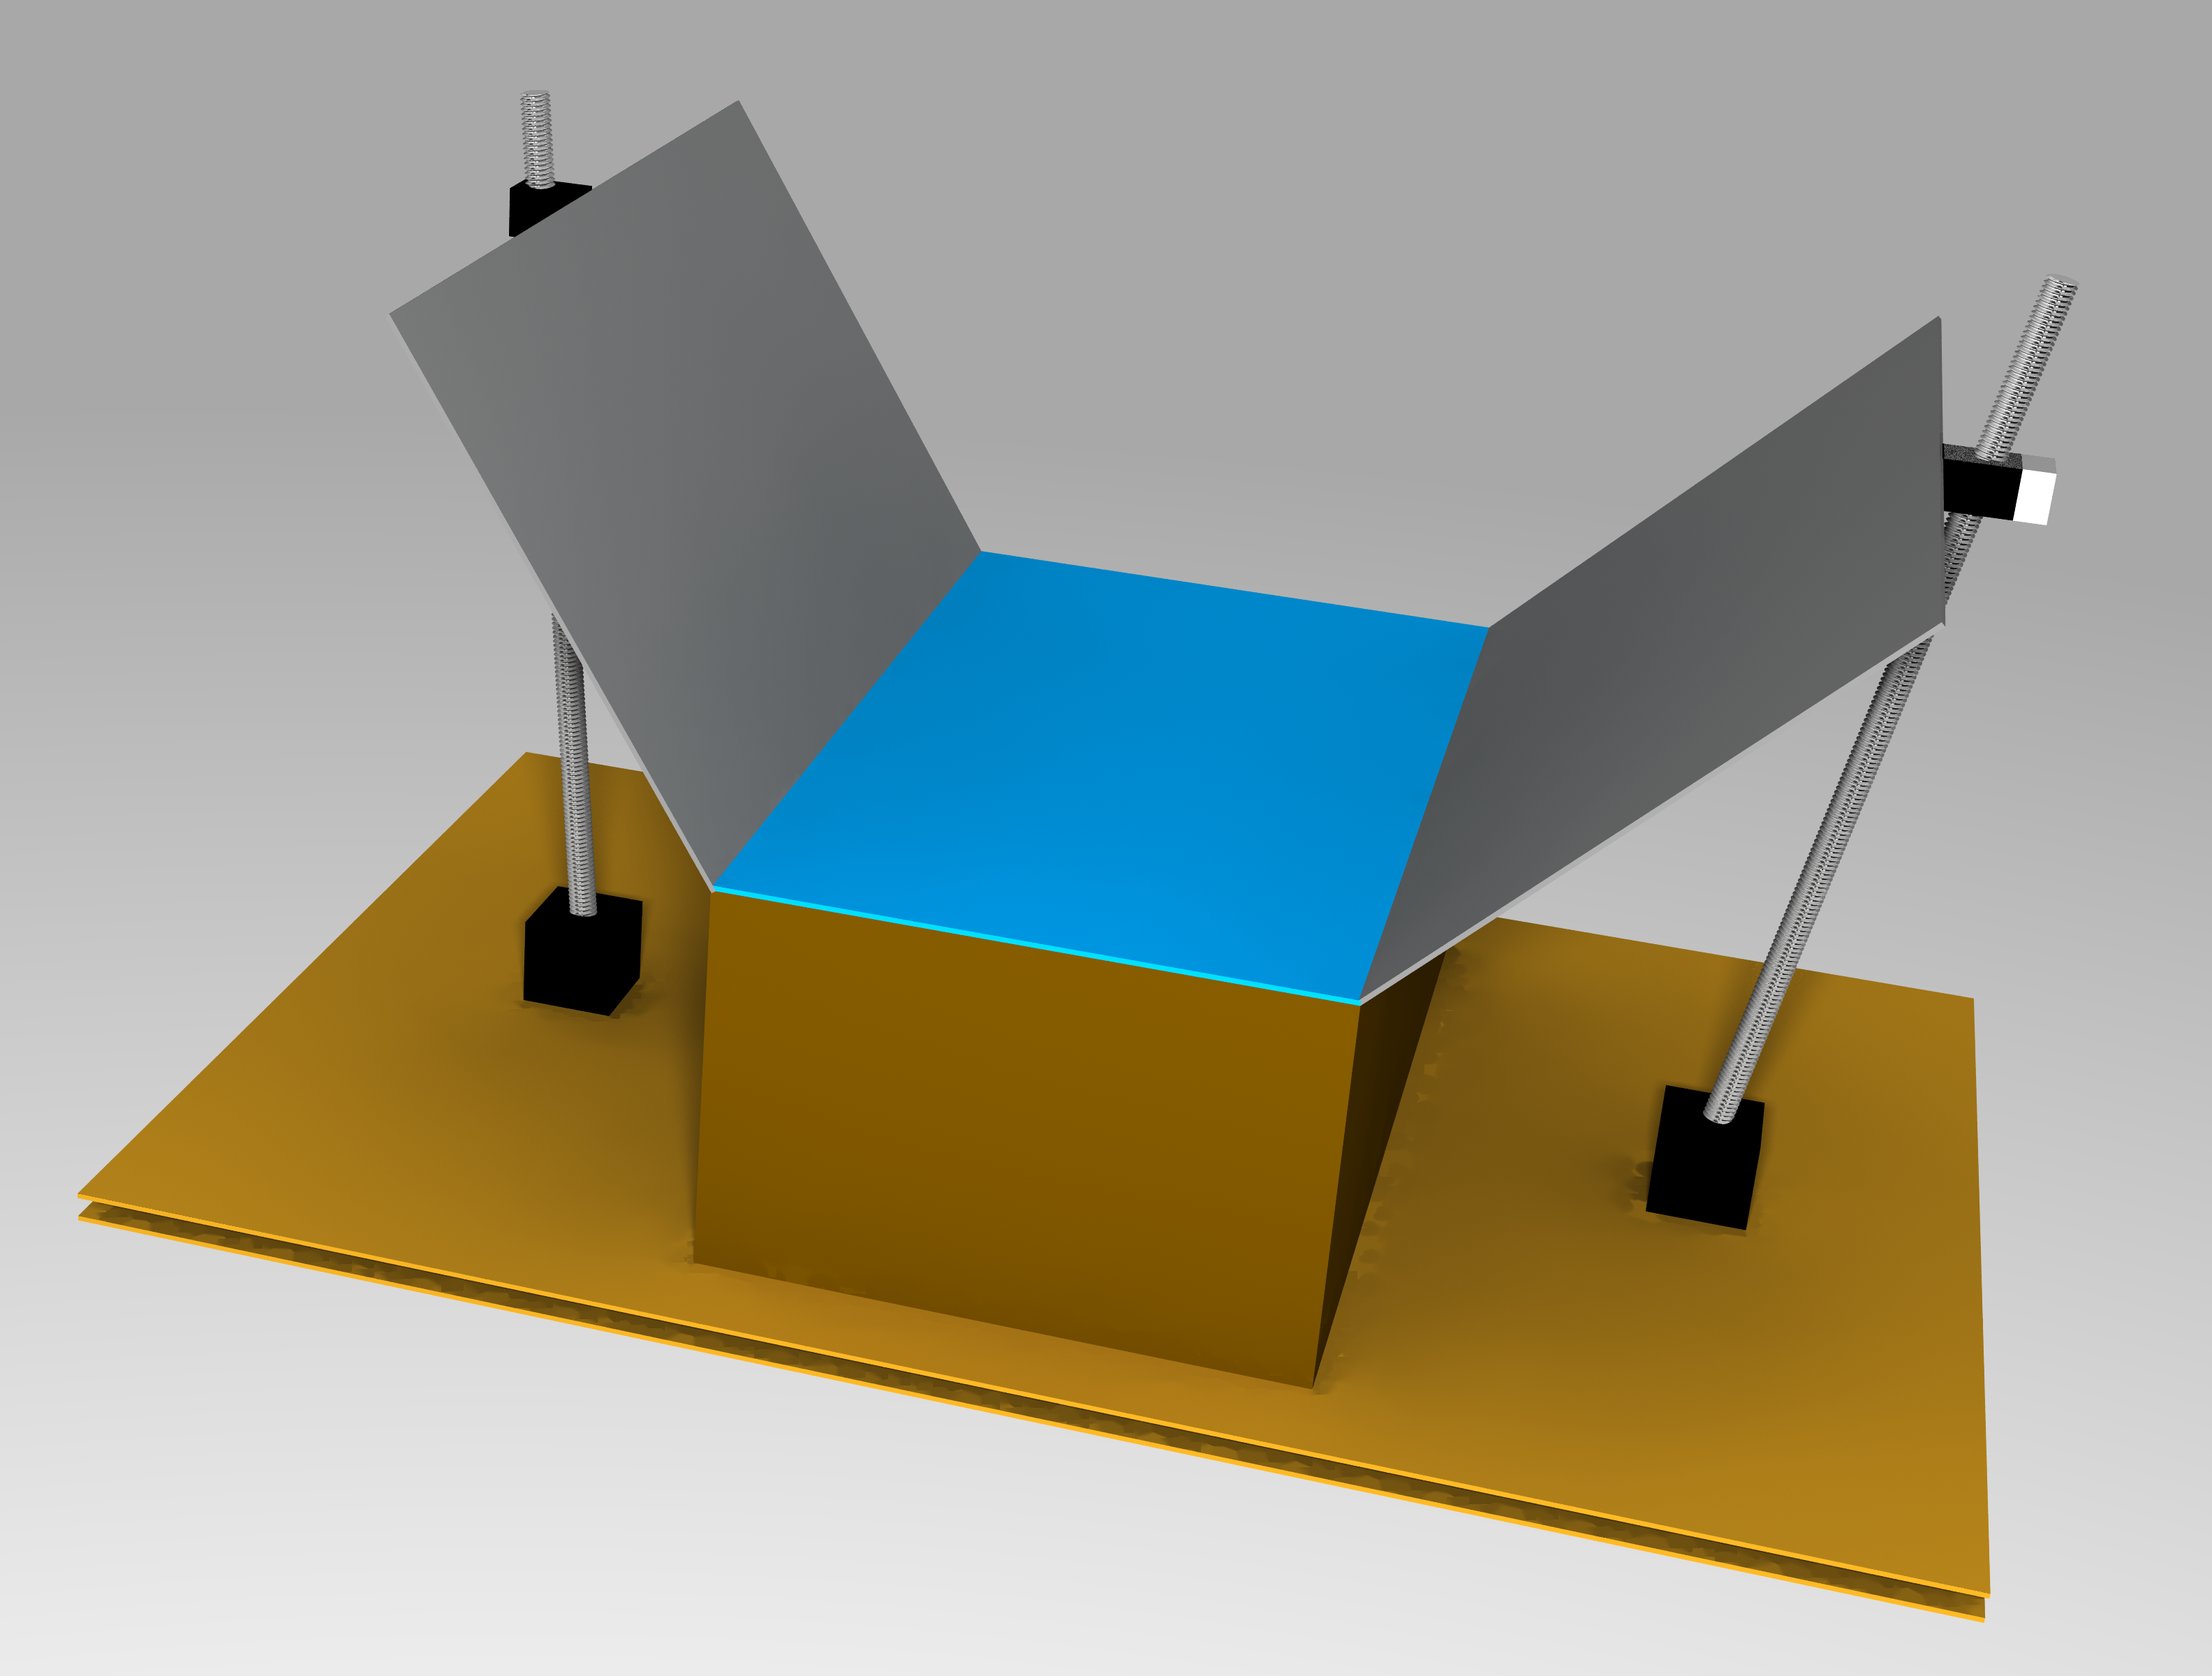
\includegraphics[width=\textwidth-100pt]{Draws/3D_render_cut.png}
        \caption{Modello generico struttura di base}
    \end{figure}
    
    \vfill


\section{Schema a blocchi}

\begin{figure}[h]
\centering
    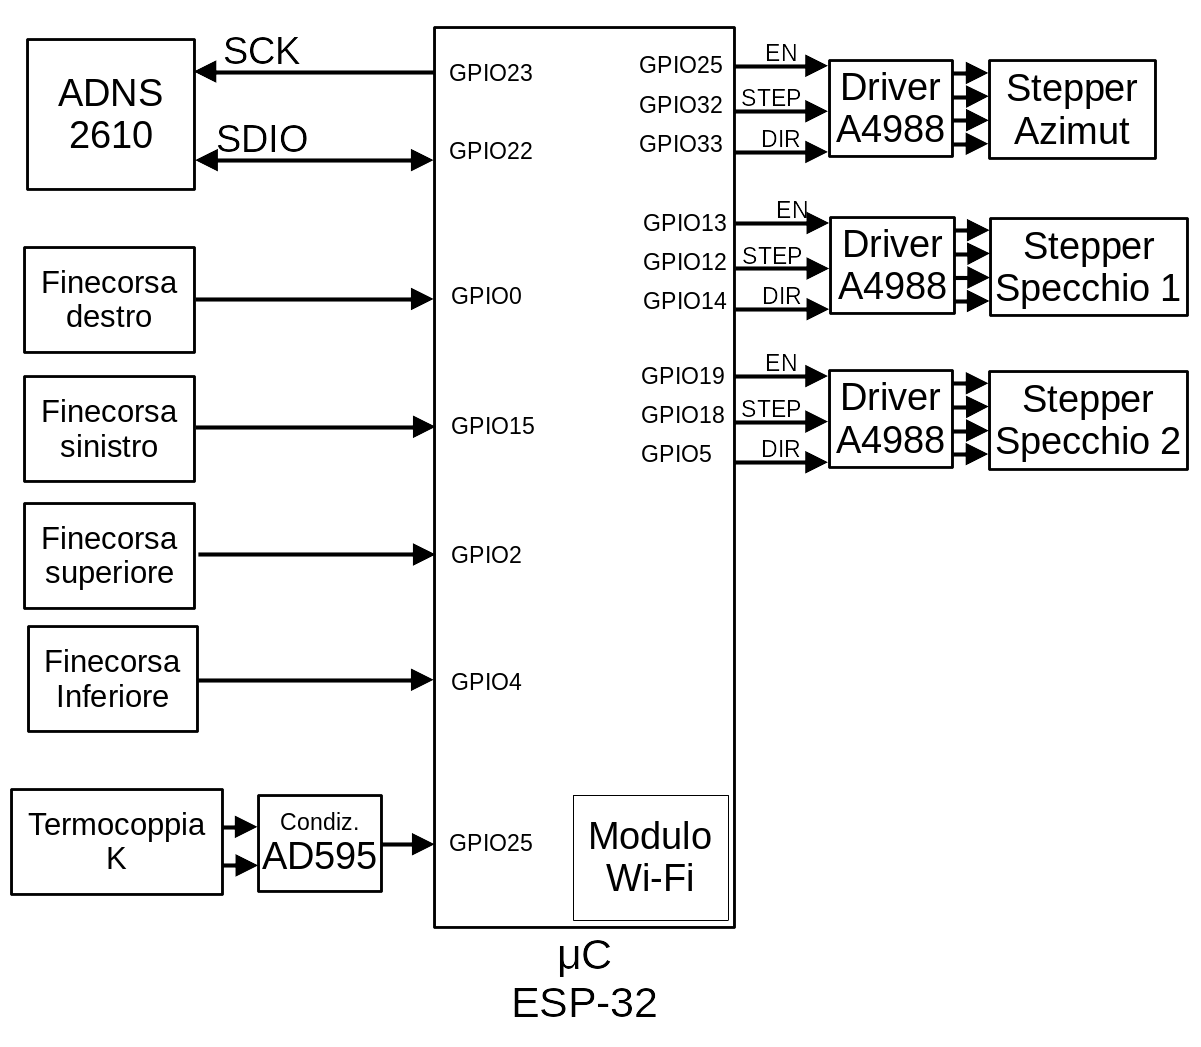
\includegraphics[width=\textwidth-30pt]{Draws/Block_diagram.png}
    \caption{Schema a blocchi}
\end{figure}

I pin indicati a destra nel diagramma (GPIO25, GPIO32, GPIO33, GPIO13, GPIO12, GPIO14, GPIO19, GPIO18 e GPIO5) sono uscite, mentre i pin indicati a sinistra (GPIO23, GPIO0, GPIO15, GPIO2, GPIO4, GPIO25) sono input, unica eccezione il GPIO 22, che, come trattato in seguito nella sezione \ref{adns2610_protocol}, per la natura del protocollo seriale implementato dal sensore ADNS2610 richiede la possibilità di scambiare dati in modo bidirezionale. Tutti gli ingressi e le uscite utilizzate sono digitali, fatta eccezione del GPIO25 che è collegato internamente ad un ADC a 12 bit integrato nel ESP-32 (per cui non sono necessari ulteriori componenti esterni per effettuare la conversione).\\
Tutti i componenti direttamente utilizzati dall'ESP-32 sono compatibili con la logica 0V - 3.3V del microcontrollore e hanno assorbimenti molto limitati (inferiori a pochi mA).\\

Il modulo Wi-Fi è interno al chip dell'ESP-32 e dunque non richiede collegamenti con i pin esterni.

\/*
Si assumono i finecorsa collegati in pulldown e con uscita allo stato alto quando premuti.\\

\begin{figure}[h]
\centering
    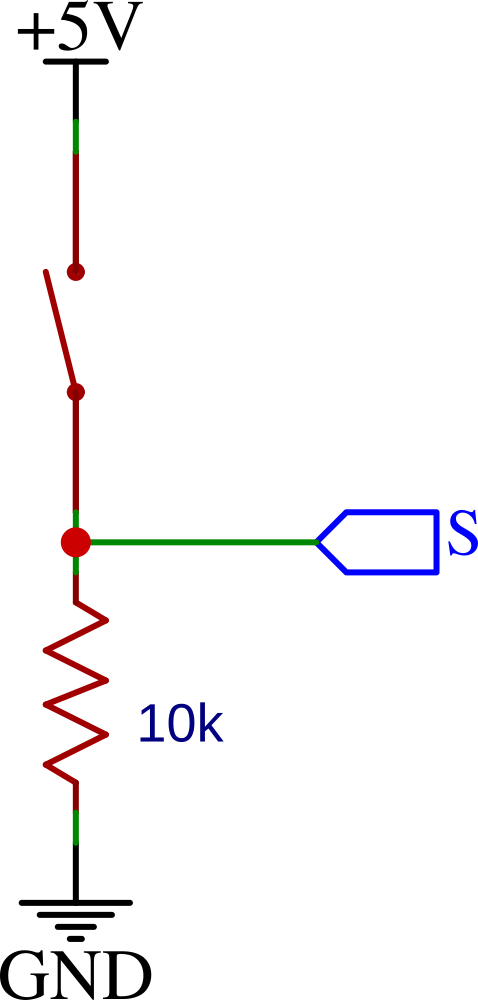
\includegraphics[width=55pt]{Draws/Pull_down.png}
    \caption{Pulldown finecorsa}
\end{figure}
*/

Lo schema circutale completo è riportato di seguito.
\begin{figure}[h]
\centering
    \includegraphics[width=\textwidth]{Draws/Schematic.png}
    \caption{Schema circuitale}
\end{figure}

L'alimentazione del sistema può esse fornita da un pannello solare per rendere il dispositivo indipendente dalla rete elettica; la logica di controllo richiede una tensione di 5V, mentre i motori di 12V, per cui è stato necessario impiegare due regolatori di tensione LM2596. Essi sono convertitori step-down DC-DC regolabili, che permettono di ottenere in uscita una tensione inferiore a quella in ingresso in modo efficiente, limitando le dispersioni di calore.


\newpage

\section{Descrizione componenti}
    \subsection{Microcontrollore}
    Per la realizzazione di questo sistema di controllo è stato scelto di utilizzare un ESP-32, un microcontrollore a 32 bit con ingressi e uscite compatibili con la logica TTL.\\
    Questo microcontrollore (come il suo predecessore ESP8266) è spesso impiegato in applicazioni IoT, anche in ambito professionale, per la connessione wifi (e bluetooth per quanto riguarda l'ESP-32) integrata in un unico chip a basso costo, permettendo ai diversi dispositivi di comunicare tra loro.\\
    Per semplicità costruttiva di seguito ci si riferirà alla specifica implementazione me\-dian\-te la scheda di prototipazione rapida NodeMCU.
    
    \subsection{Motori}
    Dovendo regolare con accuratezza la rotazione dei motori, per il controllo di azimuth e inclinazione, si è deciso di impiegare dei motori passo-passo, o stepper, in particolare il modello NEMA-17.\\
    Questi attuatori sono motori ad impulsi, in quanto composti da bobine disposte in modo tale che, se eccitate in ordine opportuno, permettono di produrre una rotazione dell'asse inferiore a 1.8° per ogni step.\\
    Il principio di funzionamento è schematizzato nell'immmagine seguente.\\
    
    
    
    \begin{figure}[h]
    \centering
        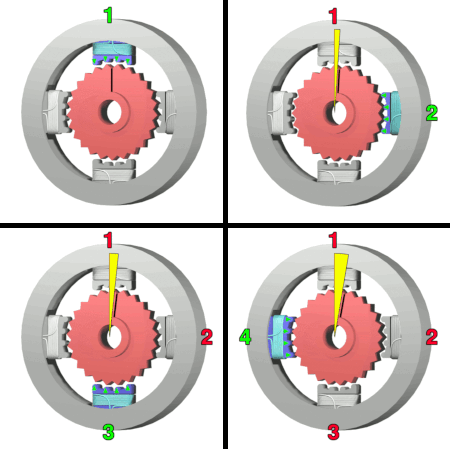
\includegraphics[width=200pt]{Draws/Animations/StepperMotor.png}
        \caption{Fasi motore passo-passo, Wikimedia Commons \protect\footnotemark}
    \end{figure}
    
    \footnotetext{Questa immagine è tratta e modificata da Wikimedia Commons, informazioni riguardo l'autore originale, modifiche successive e licenza GNU Free Documentation License possono essere reperite al seguente link: commons.wikimedia.org/wiki/File:StepperMotor.gif}
    
    
        \subsubsection{Controllo di potenza}
        Per il controllo dell'attivazione delle bobine si è scelto di utilizzare il modulo A4988 (molto diffuso nelle macchine a controllo numerico hobbistiche), che permette il controllo della rotazione del motore mediante un segnale di direzione (orario/antiorario) e un segnale di step.\\
        La logica di attivazione degli avvolgimenti del motore è gestita dell'integrato mediante due ponti H a fet, uno per bobina, che permettono la regolazione della potenza ad ogni avvolgimento.\\
        Il funzionamento interno, come mostrato dal costruttore nel datasheet, può essere schematizzato con il seguente diagramma a blocchi.\\
        \begin{figure}[h]
        \centering
            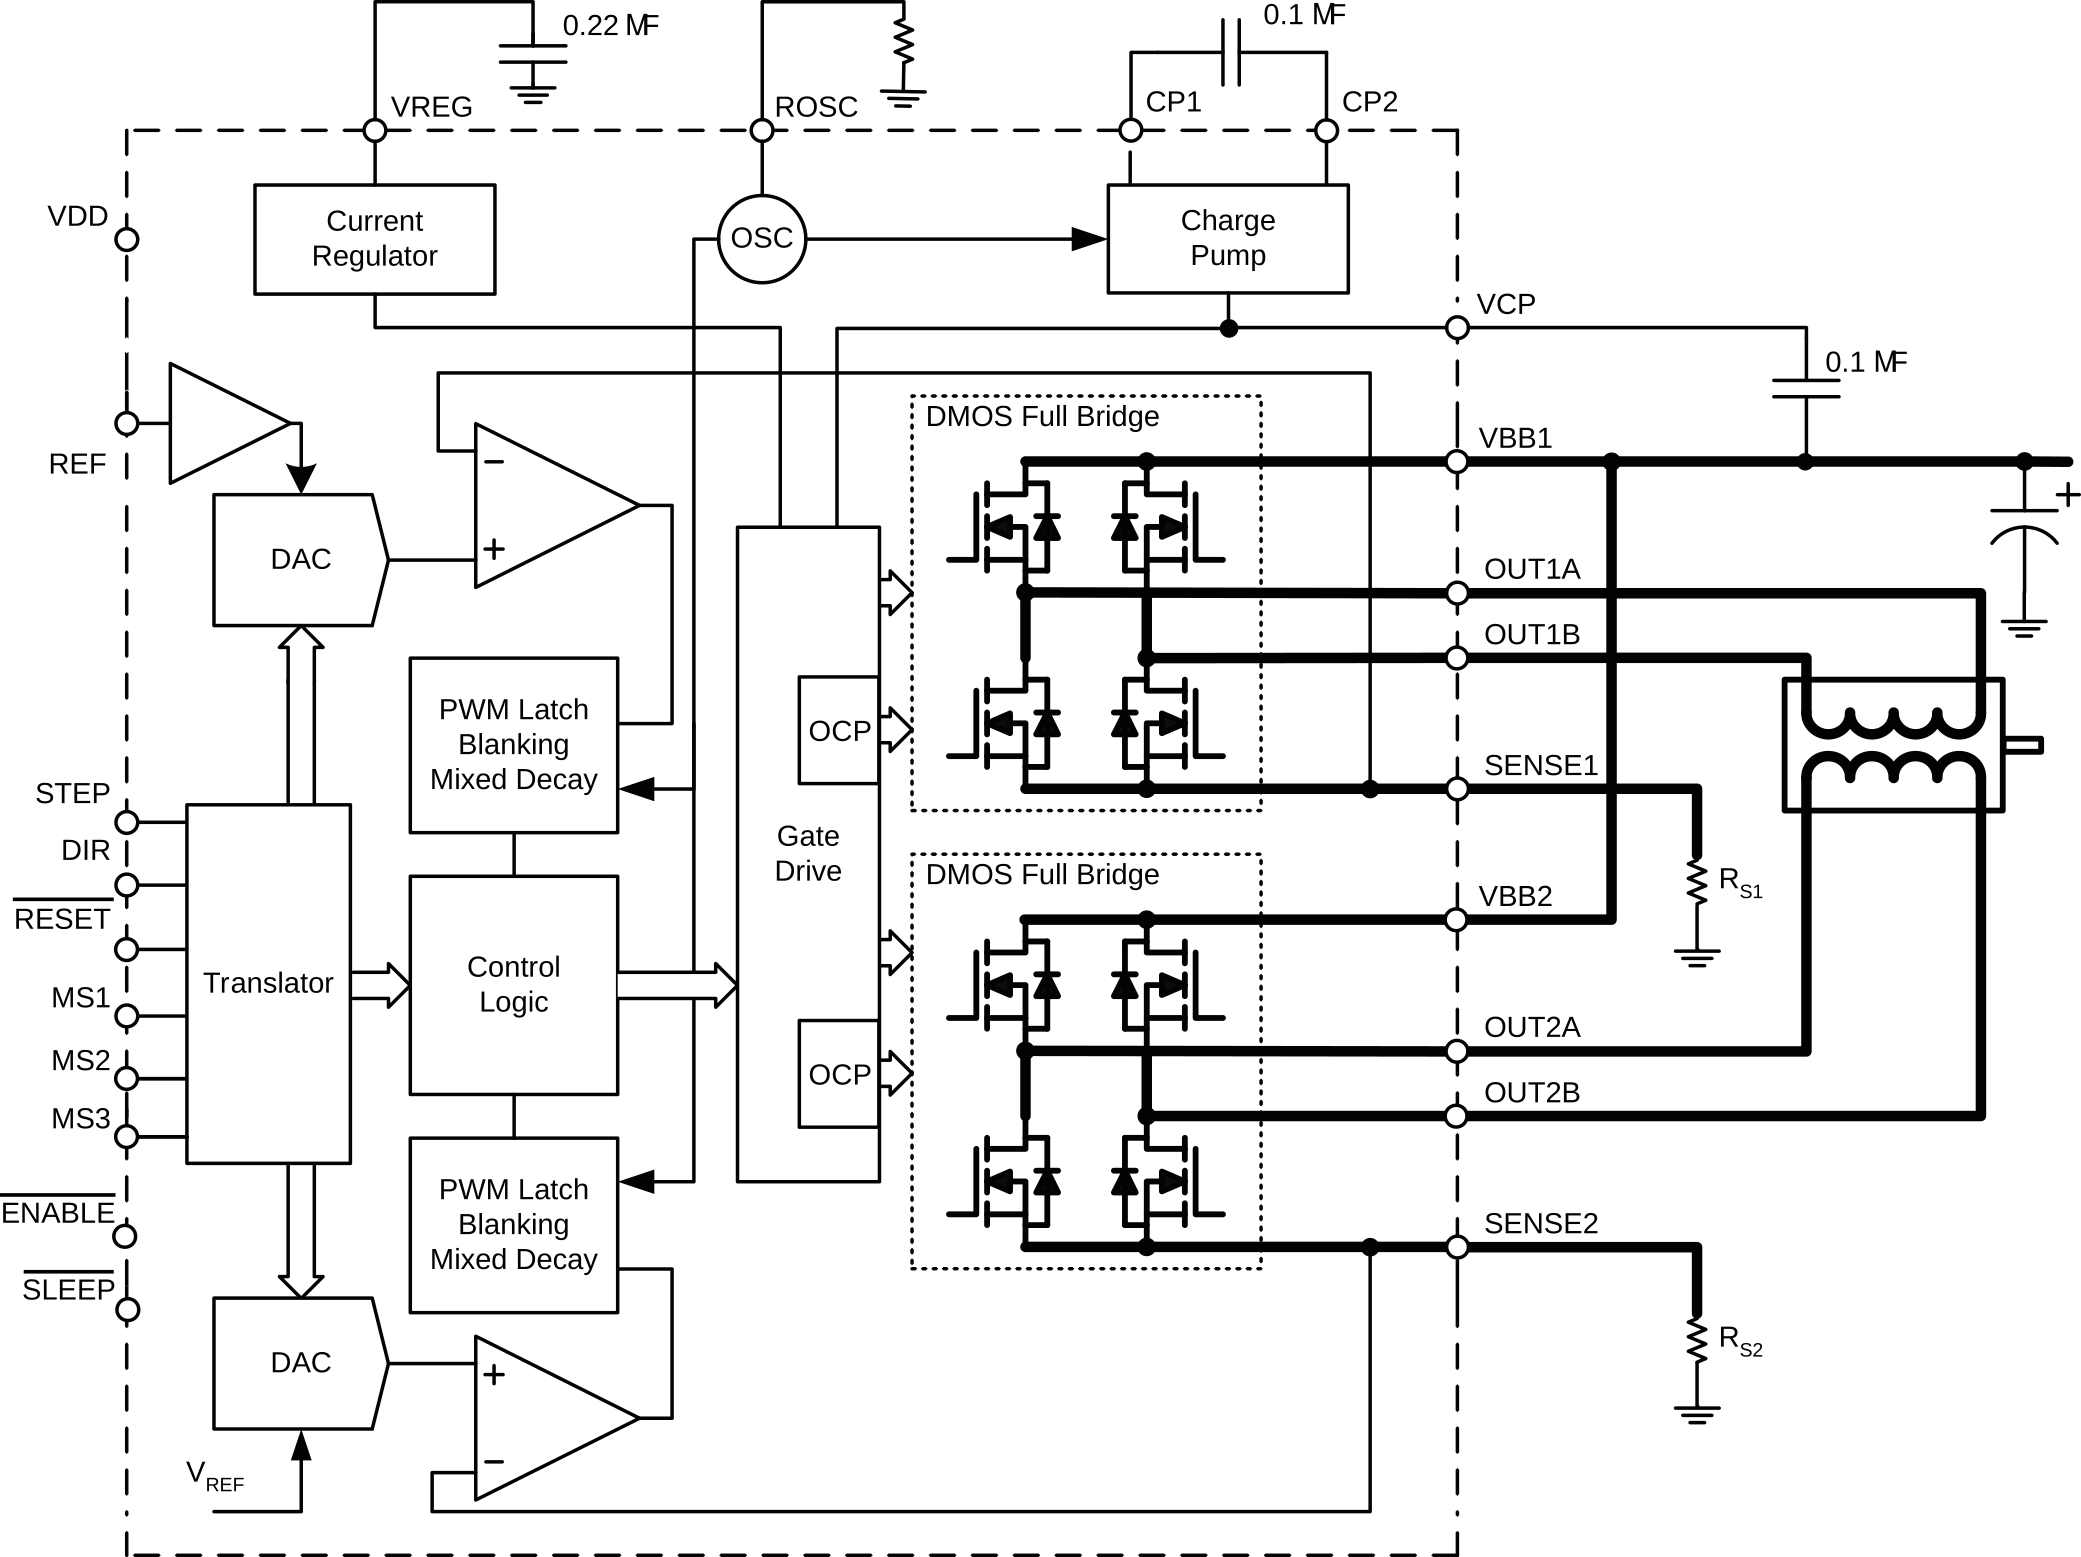
\includegraphics[width=320pt]{Draws/A4988_functional_diagram.png}
            \caption{Diagramma funzionamento interno A4988, datasheet}
            \label{fig:A4988_diagram}
        \end{figure}
        
        \noindent
        Gli ingressi $MS_1$, $MS_2$ e $MS_3$ permettono la selezione del rapporto di microstepping, infatti oltre alla modalità full-step, in cui le singole bobine vengono eccitate con controllo ON-OFF in successione, è possibile realizzare un controllo micro-stepping con l'attivazione progressiva delle bobine consecutive, permettendo di mantenere il rotore tra due stati successivi, garantendo una maggiore fluidità di movimento, riducendo oscillazioni, vibrazioni e dunque sollecitazioni meccaniche della struttura fisica.\\
        Con riferimento all'immagine di Fig. \ref{fig:A4988_diagram} si può osservare che il dispositivo permette di regolare la coppia massima del motore mediante la regolazione di una tensione di riferimento che agisce sulla corrente massima che viene fornita alle bobine (misurata dalle resistenze di shunt $R_{s1}$ e $R_{s2}$ che forniscono un feedback al sistema di controllo).

        \vspace{0.1cm}


    \subsection{Termocoppia}\label{thermocouple}
    Per la rilevazione della temperatura si è scelto di utilizzare una termocoppia di tipo K a giunzione Chromel-Alumel (leghe metalliche a base di nichel), sensore molto diffuso che premette di misurare temperature nel range da circa -200 °C a oltre 1300 °C, con una sensibilità di $41 \frac{\mu V}{\degree C}$.\\
    Le termocoppie sfruttano l'effetto Seebeck, un effetto termoelettrico che produce una differenza di potenziale tra due punti di un materiale conduttore proporzionale alla differenza di temperatura tra i due punti (detti guinzione calda e giunzione fredda); l'intensità di questo effetto varia a seconda del materiale in considerazione e quindi, utilizzando due maetalli differenti, è possibile calcolare la temperatura del giunto caldo nota la differenza di potenziale e la temperatura del giunto freddo.\\
    Per rendere apprezzabili tali variazioni di tensione è necessario impiegare un amplificatore da strumentazione, in particolare si è scelto l'AD595, che garantisce la compensazione interna della temperatura della giunzione fredda e fornisce in uscita una tensione proporzionale alla tempreatura secondo la relazione:
    \begin{equation}\label{thermocouple_relation_AD595}
        V_{out} = T \cdot 10 \frac{mV}{\degree C}
    \end{equation}
    Nella sezione \ref{conditioning} si tratterà più approfonditamente il condizionamento di questo segnale per sfruttare l'intero range dell'ADC del microcontrollore.
    
    
    \subsection{Sensore ottico}\label{optical_sensor}
    Il sensore principale di questo sistema di controllo è l'ADNS-2610, che viene utilizzato dal microcontrollore per calcolare l'azimuth e l'elevazione relativi del sole.\\
    
    \begin{figure}[h]
        \centering
        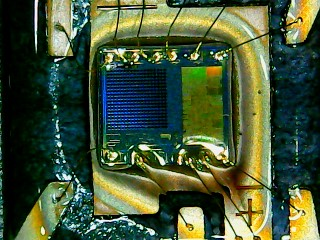
\includegraphics[width=250pt]{Draws/ADNS-2610_die/WIN_20210501_17_42_53_Pro.jpg}
        \caption{Sensore ADNS-2610}
        \label{fig:ADNS2610_die}
    \end{figure}
   
   
    Questo integrato nasce come sensore per mouse ottici, che dispongono di una fotocamera a bassa risoluzione e confrontano le immagini di due frame successivi per individuare lo spostamento relativo alla superficie sottostante, nella porzione di sinistra della figura \ref{fig:ADNS2610_die} si osserva la matrice 18x18 degli elementi fotosensibili (l'immagine è stata realizzata con un ingrandimento e l'area effettiva coperta dalla griglia è di circa 2 $mm^2$).\\
    Il principio di funzionamento è identico ad una camera a foro di spillo, in cui l'immgine viene proiettata sullo schermo fotosensibile attraverso un foro circolare di piccole dimensioni.
    
    \begin{figure}[h]
        \centering
        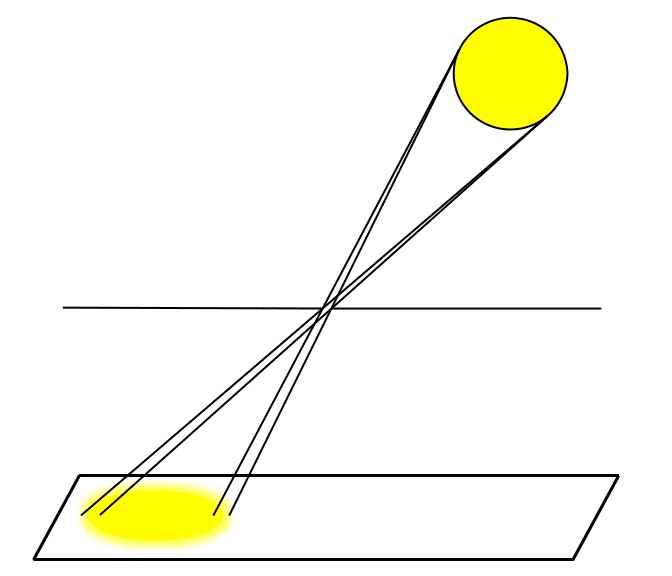
\includegraphics[width=150pt]{Draws/Pinhole_sun}
        \caption{Schema immagine stenoscopica}
        \label{fig:pinhole_sun}
    \end{figure}
    
    
    La posizione dell'immagine sullo schermo, a parità delle altre condizioni, varia al variare della distanza tra il foro e il sensore stesso, in particolare, aumentando tale distanza il dispositivo avrà un angolo di campo minore, viceversa, diminuendo la distanza foro-rivelatore, si otterrà un angolo di campo maggiore.
    
    \begin{figure}[h]
        \centering
        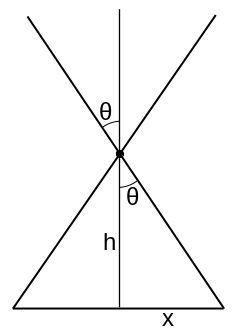
\includegraphics[width=100pt]{Draws/Pinhole_diagram}
        \caption{Diagramma camera a foro di spillo}
        \label{fig:pinhole_diagram}
    \end{figure}
    
    
    In cui la relazione tra $x$ e l'angolo $\theta$ del raggio rispetto allo zenit è:
    \begin{equation}\label{pinhole_angle_relation}
        x = h \cdot tan(\theta)
    \end{equation}
    
    
    Maggiori dettagli riguardo l'interfacciamento in protocollo con il microcontrollore sono forniti nella sezione \ref{adns2610_protocol}.
    
    %\subsection{Interfaccia web}
    
 
\section{Condizionamento segnale sensore temperatura}\label{conditioning}
    Considerata l'uscita del AD595 descritta dall'equazione (\ref{thermocouple_relation_AD595}) nella sezione \ref{thermocouple} e considerata la risoluzione di 12 bit degli ADC del microcontrollore, si ottiene una minima variazione apprezzabile (idealmente) inferiore a 0.12 °C. Per questo motivo non è necessario realizzare un secondo condizionamento del segnale, in quanto tale valore di incertezza è trascurabile rispetto alle temperature da misurare e alle altre fonti di errore presenti; per maggiore completezza si riporta comunque un possibile condizionamento di tale segnale. \\
    
    \vspace{0.2cm}
    
    \noindent
    Si limiti il range di interesse da 15°C a 300°C in cui rientra la regolare temperatura di un forno solare. Secondo la relazione (\ref{thermocouple_relation_AD595}) l'uscita in tensione del sensore varierà all'interno dell'intervallo [150mV; 3.0V], mentre l'ADC integrato nel microcontrollore, con $V_{ref}$ standard, ammette ingressi nel range [0V; 3.3V]; di seguito si suppongono tutti i dispositivi impiegati come ideali. È possibile applicare un offset e successivamente un'amplificazione opportunamente calcolati di seguito.
        \begin{equation}\label{offset}
            {V_{offset}} = V_{Smin} - V_{ADCmin} = 150 mV
        \end{equation}
        
        \begin{equation}\label{amplification}
            A = \frac{V_{ADCmax}-V_{ADCmin}}{V_{Smax} - V_{Smin}} \simeq 1.16
        \end{equation}
        Tali valori possono essere ottenuti utilizzando un amplificatore operazionale in configurazione differenziale come segue.

        \noindent
        \begin{center}
            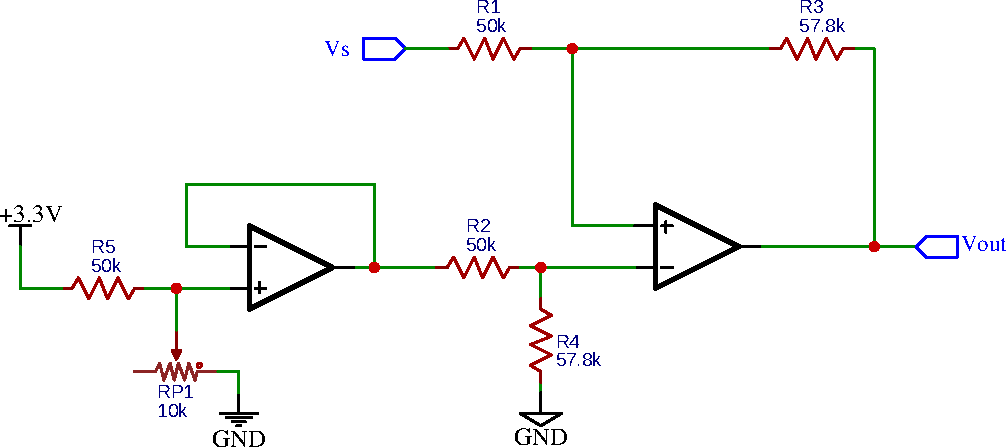
\includegraphics[
                page=1,
                width=\textwidth-150pt,
                keepaspectratio
            ]{Draws/Schematic_Elaborato_2021-05-15_differential.pdf}
        \end{center}
                
        \noindent
        In cui il potenziometro (o trimmer) $RP_1$ deve essere opportunamente regolato in fase di calibrazione per ottenere l'offset corretto.\\
        Essendo $R_1=R_2$ e $R_3=R_4$ l'amplificazione risulta $A = \frac{R_3}{R_1} \simeq 1.16$, stesso valore ottenuto sostituendo i rispettivi valori numerici nell'equazione (\ref{amplification}). Riguardo alle due resistenze da $57.8 k\Omega$, tale può essere ottenuto dalla serie di una resistenza da $56 k\Omega$ e da $1.8 k\Omega$, entrambi valori appartenenti alla serie E12.\\
        Combinando le equazioni (\ref{thermocouple_relation_AD595}), (\ref{offset}) e (\ref{amplification}), la funzione di trasferimento dell'amplificatore differenziale e considerata la conversione dell'ADC a 12 bit dell'ESP-32 (valore da 0 a 4095), si ottiene:
        \begin{equation}
            Val_{ADC} = \left( T \cdot 10 \left[ \frac{mV}{\degree C} \right] - 150 [mV] \right) \cdot \frac{57.8}{50} \cdot \frac{4095}{3.3[V]} \simeq \left( \frac{T}{1 [\degree C]} - 15 \right) \cdot  14.345
        \end{equation}
        
        \noindent
        chiaramente approssimato all'intero, da cui si ricava
        
        \begin{equation}
            T = \left( \frac{Val_{ADC}}{14.345} + 15 \right) [\degree C]
        \end{equation}
    
        \noindent
        L'aggiunta di questo condizionamento richiede inoltre ulteriori componenti per la generazione dell'alimentazione duale per l'operazionale, quindi, in aggiunta a quanto già discusso all'inizio di questa sezione, non è stato ritenuto necessario impiegare condizionamenti successivi all'integrato AD595.

\newpage
\section{Cenni matematici}
    \subsection{Sistema coordinate cartesiane - polari}
    Si ricorda che è possibile definire in modo univoco un punto A sul piano cartesiano mediante le sue coordinate $(x_A, y_A)$. Lo stesso punto A può anche essere descritto univocamente dalla distanza $r$ dal centro e dall'angolo $\alpha$ che esso forma con il centro e il semiasse positivo delle ascisse. È possibile ottenere la rapprentazione cartesiana dalle coordinate polari e viceversa secondo le relazioni:
    
    \begin{equation}
        \begin{split}
        x_A = r \cdot \cos\alpha \\
        y_A = r \cdot  \sin\alpha
        \end{split}
    \end{equation}
    
    \begin{equation}
        \begin{split}
        r = \sqrt{x_A^2 + y_A^2} \\
        \alpha = atan \left(\frac{y_A}{x_A} \right)
        \end{split}
    \end{equation}
    
    \begin{figure}[h]
    \centering
        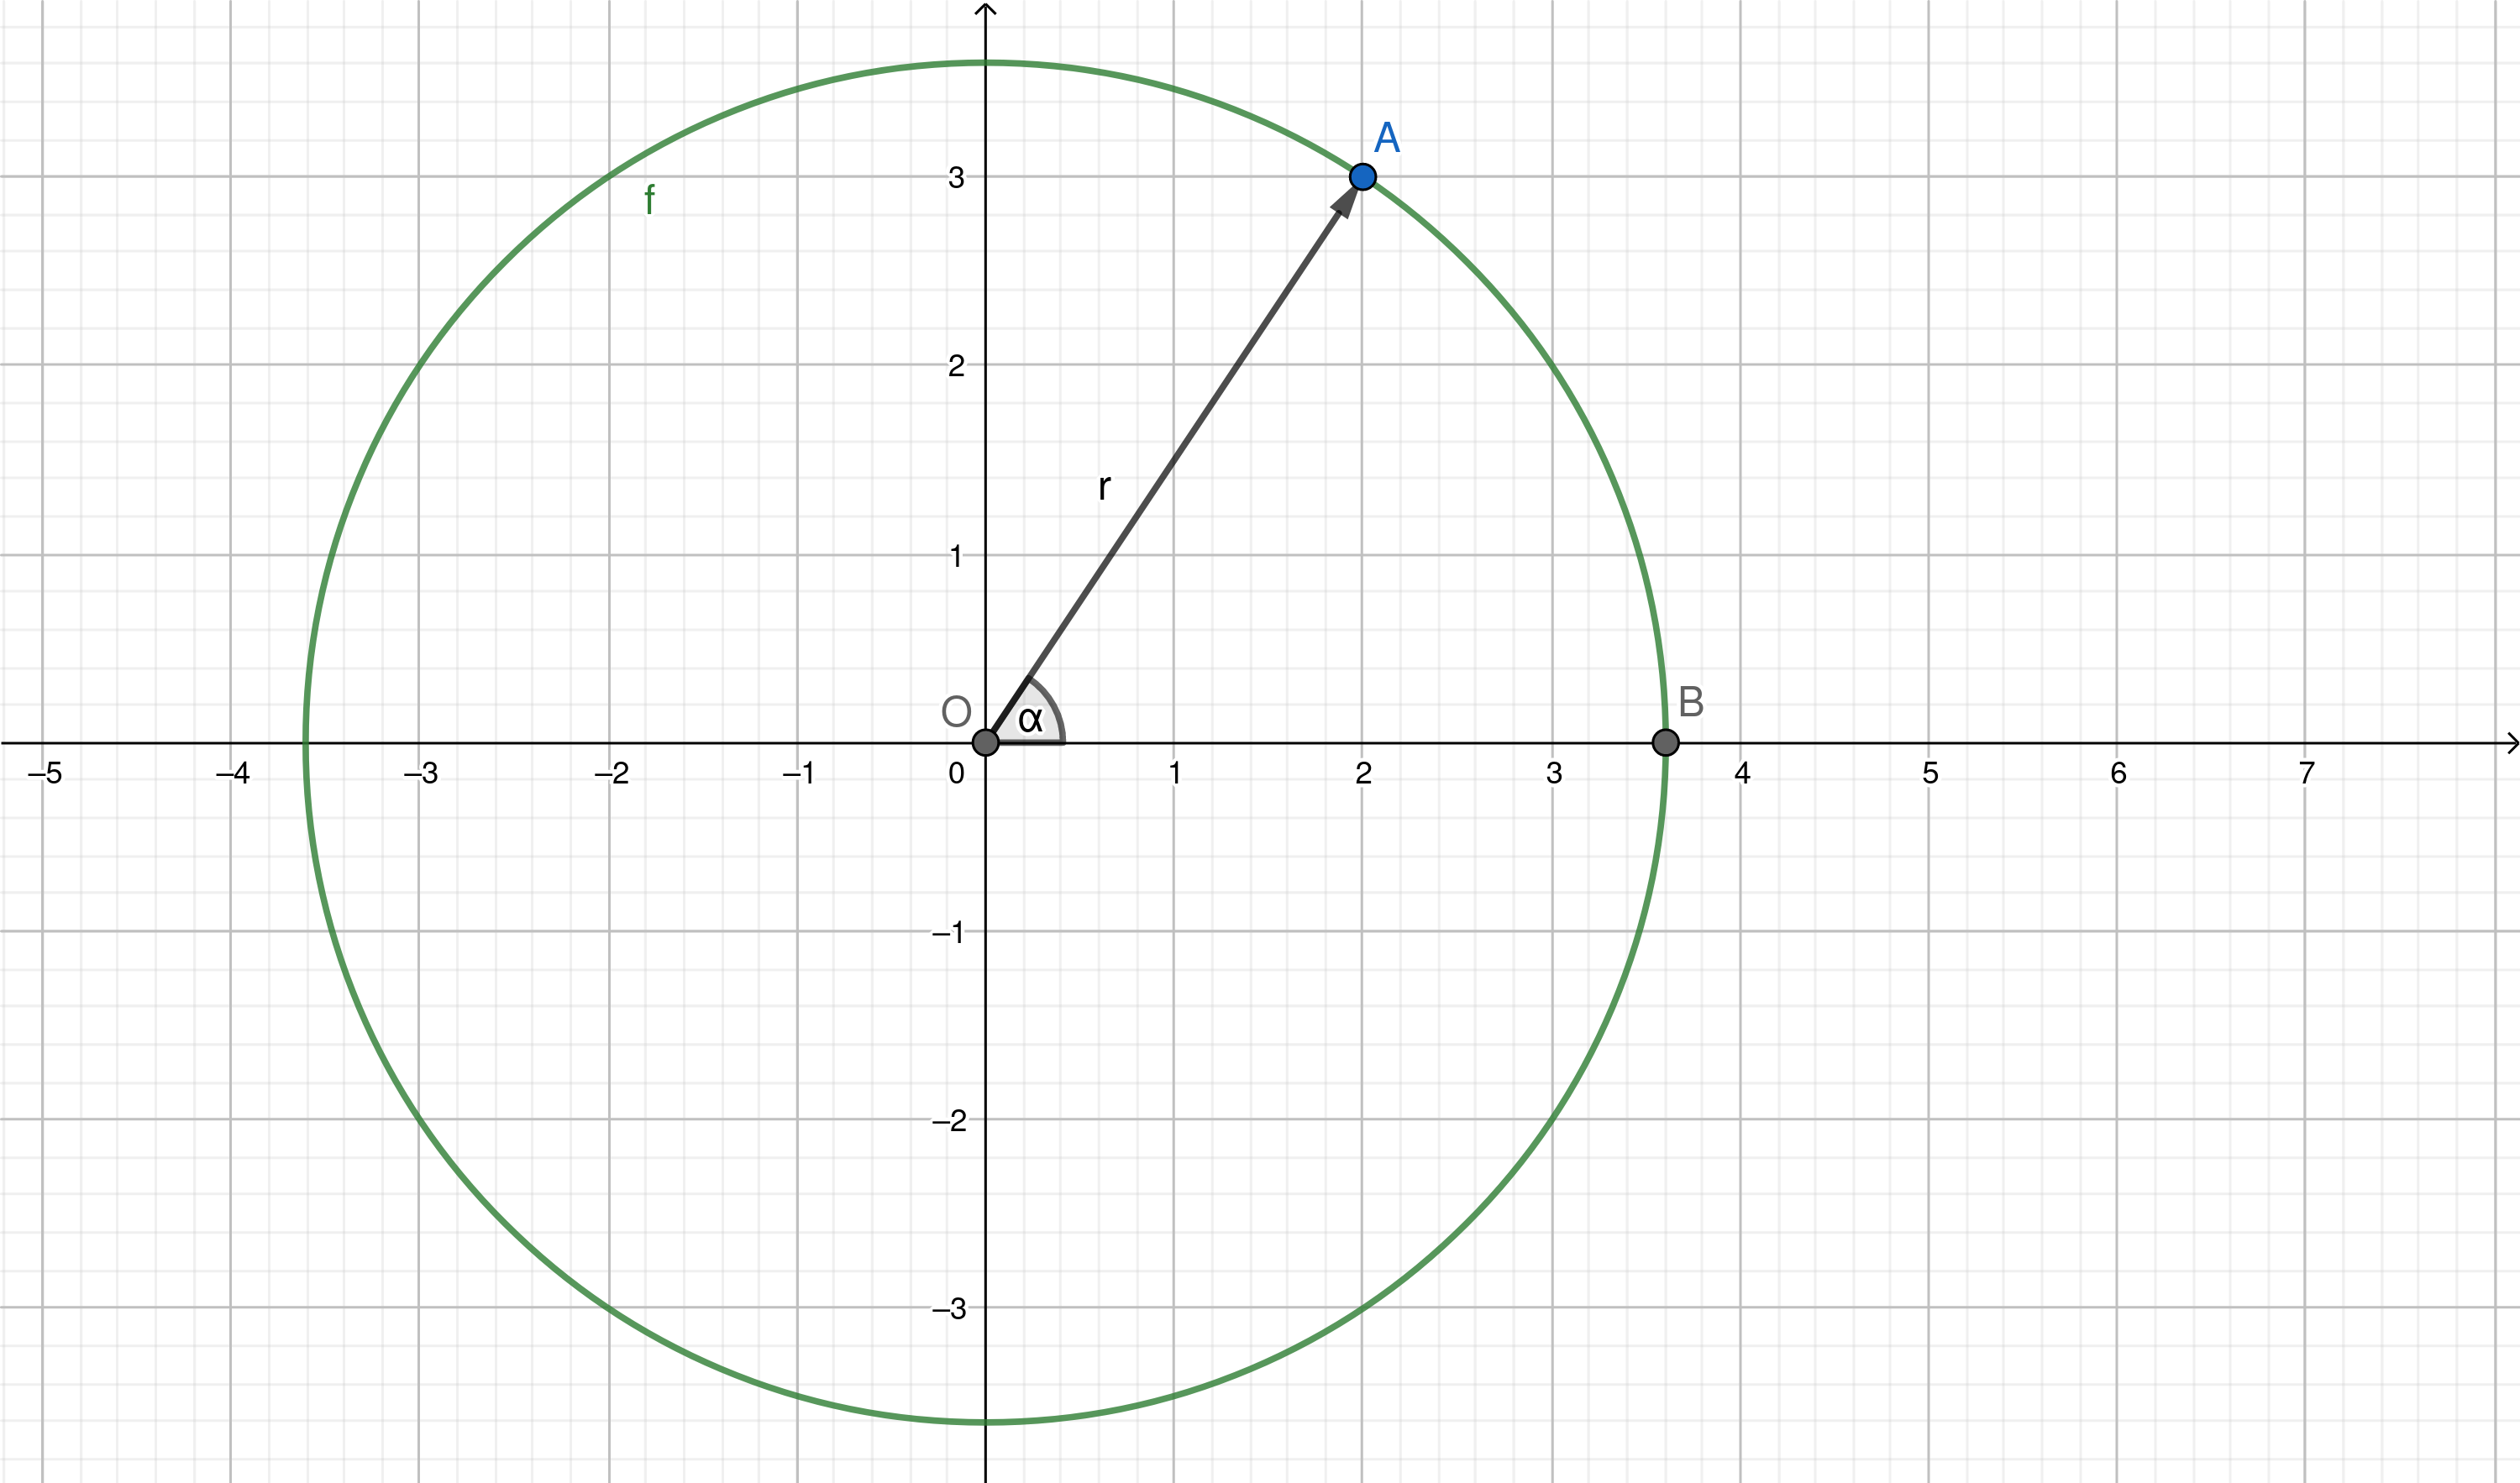
\includegraphics[width=190pt]{Draws/geogebra-export_polar_circle.png}
        \caption{Rappresentazione coordinate polari su piano cartesiano, geogebra}
    \end{figure}
    
    In particolare, una volta determinata la posizione del centro del sole nell'immagine acquisita, ed espresso tale punto in coordinate polari $(r, \alpha)$, $r$ è direttamente legato all'elevazione effettiva del sole secondo la relazione (\ref{pinhole_angle_relation}), mentre $\alpha$ indica la diffetenza tra l'azimuth del sole e la posizione attuale della base girevole. Si osserva, infatti, che le due quantità possono essere trattate indipendentemente, in quanto ruotando la base varierà $\alpha$, mentre $r$ sarà, idealmente, costante (il centro si muove lungo una circonferenza di raggio $r$); viceversa, una variazione della sola elevazione non varia il valore di $\alpha$ (il punto si muove su uno stesso raggio della circonferenza originale).
    
    
    \subsection{Relazioni trigonometriche}
    Per ottimizzare la potenza assorbita dal forno si vuole che la totalità della luce che investe gli specchi venga riflessa all'interno del forno, attraverso il vetro trasparente posto sulla faccia sueriore della scatola. La situazione può essere schematizzata come mostrato nella figura \ref{sun_reflection}.

    \begin{figure}[h]
    \centering
        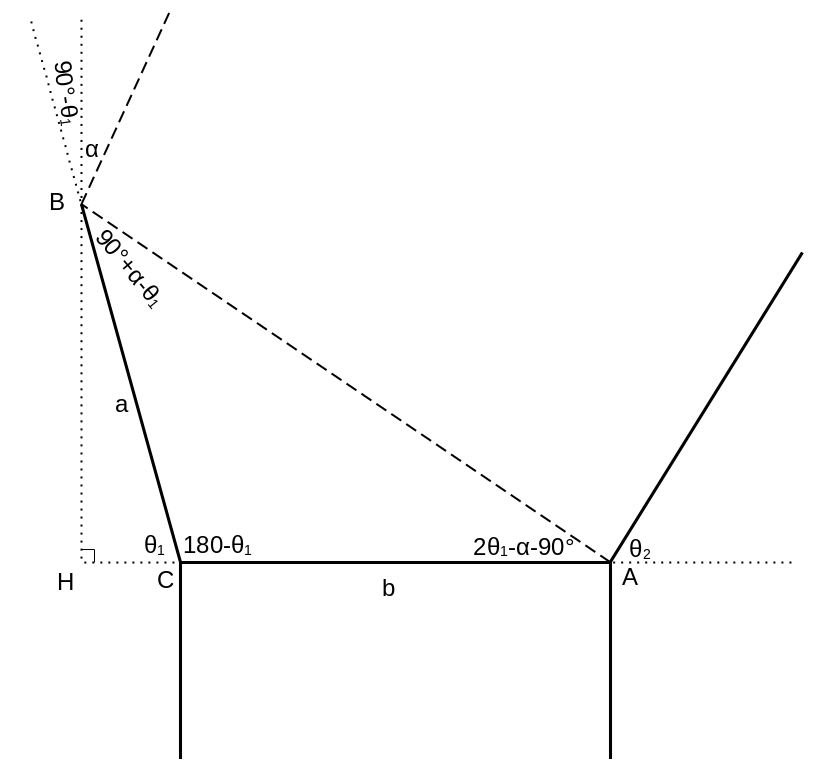
\includegraphics[width=300pt]{Draws/Reflection_schematics_trig.png}
        \caption{Schema riflessioni raggi solari}
        \label{sun_reflection}
    \end{figure}
    
    \noindent
    Dal rispetto del teorema di Carnot e dalle relazioni trigonometriche nei triangoli rettangoli si ottiene:
 
\/*
    \begin{equation}
        \sqrt{a^2 + b^2 - 2 a b \cos(\pi-\theta_1)}  \cdot \sin \left(2 \theta_1 - \alpha - \frac{\pi}{2} \right) = a \cdot \sin(\theta_1)
    \end{equation}

    \noindent
    Che può essere riscritto come:
*/

    \begin{equation}
        \sqrt{a^2 + b^2 + 2 a b \cos(\theta_1)}  \cdot \cos(2 \theta_1 - \alpha) + a \cdot \sin(\theta_1) = 0
    \end{equation}
    
    \noindent
    In modo equivalente si ottiene
    \begin{equation}
        \sqrt{a^2 + b^2 + 2 a b \cos(\theta_2)}  \cdot \cos(2 \theta_2 + \alpha) + a \cdot \sin(\theta_2) = 0
    \end{equation}
    
    
    Risolvere algebricamente queste equazioni risulta particolarmente laborioso, sebbene non difficile, e considerato che il range di interesse si limita a $\alpha \in [0, \frac{\pi}{2})$ e $\theta_1, \theta_2 \in (0, \pi)$ si può valutare di risolvere per approssimazione tali uguaglianze per trovare il valore degli angoli cercati per uno specifico valore di $\alpha$ misurato.\\
    
    \begin{figure}[h]
    \centering
        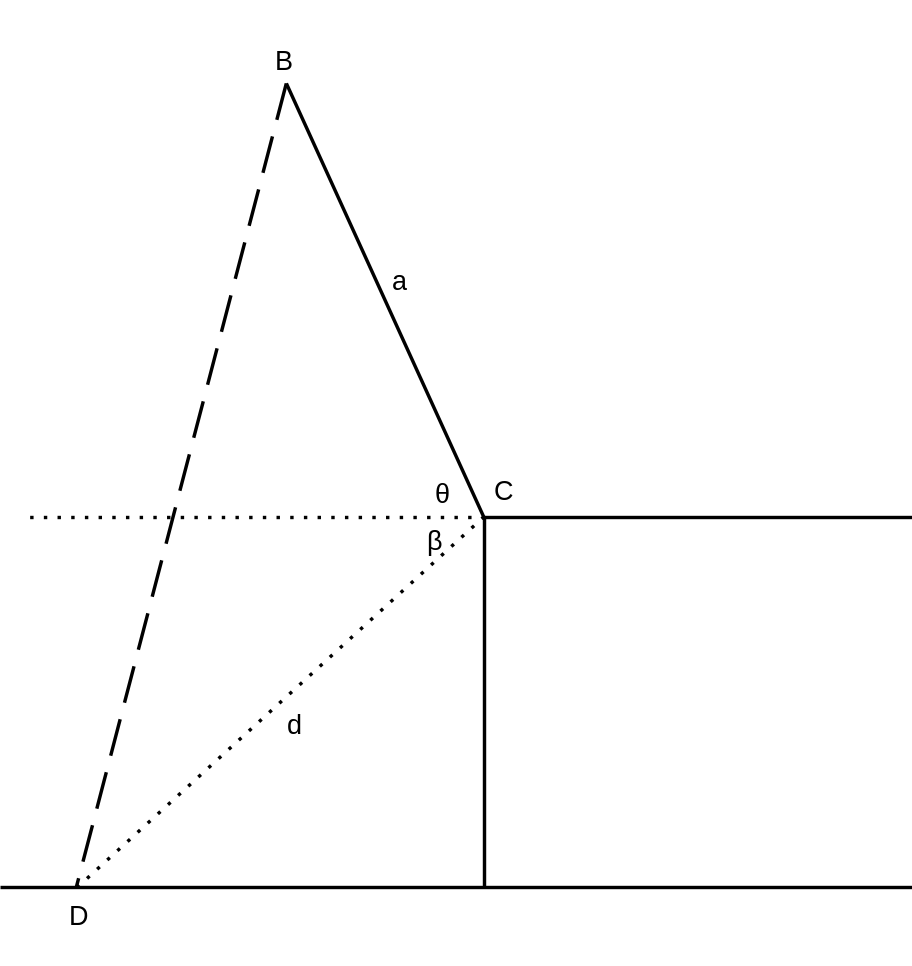
\includegraphics[width=240pt]{Draws/Linear_inclination_trig.png}
        \caption{Schema inclinazione specchi}
        \label{mirror_inclination_system}
    \end{figure}
    
    
    L'inclinazione degli specchi viene regolata mediante un sistema vite-dado, che può essere schematizzato come mostrato nella figura \ref{mirror_inclination_system}.\\
    
    In cui sia $d$ che $\beta$ sono noti, in quanto determinati dalla costruzione e $\theta$ è l'angolo calcolato in precedenza. È quindi possibile calcolare la distanza $\overline{\rm BD}$, dipendente dalla rotazione del motore, applicando nuovamente il teorema di Carnot:
    
    \begin{equation}
        \overline{\rm BD} = \sqrt{a^2 + d^2 - 2 a b \cdot \cos(\beta + \theta)}
    \end{equation}
    
    \vspace{1.5cm}
    
    Infine, nota tale distanza, è possibile calcolare la rotazione del motore per portarlo alla posizione voluta, ma è necessario conoscere anche la posizione attuale assoluta dello specchio, per questo motivo è necessario un finecorsa che all'accensione permetta al controllore di avere un riferimento assoluto (analoga alla procedura di homing per le macchine a controllo numerico).


\newpage
\section{Algoritmo}
    \subsection{Diagramma di flusso generale}
        \subsubsection{Setup}
            \begin{center}
                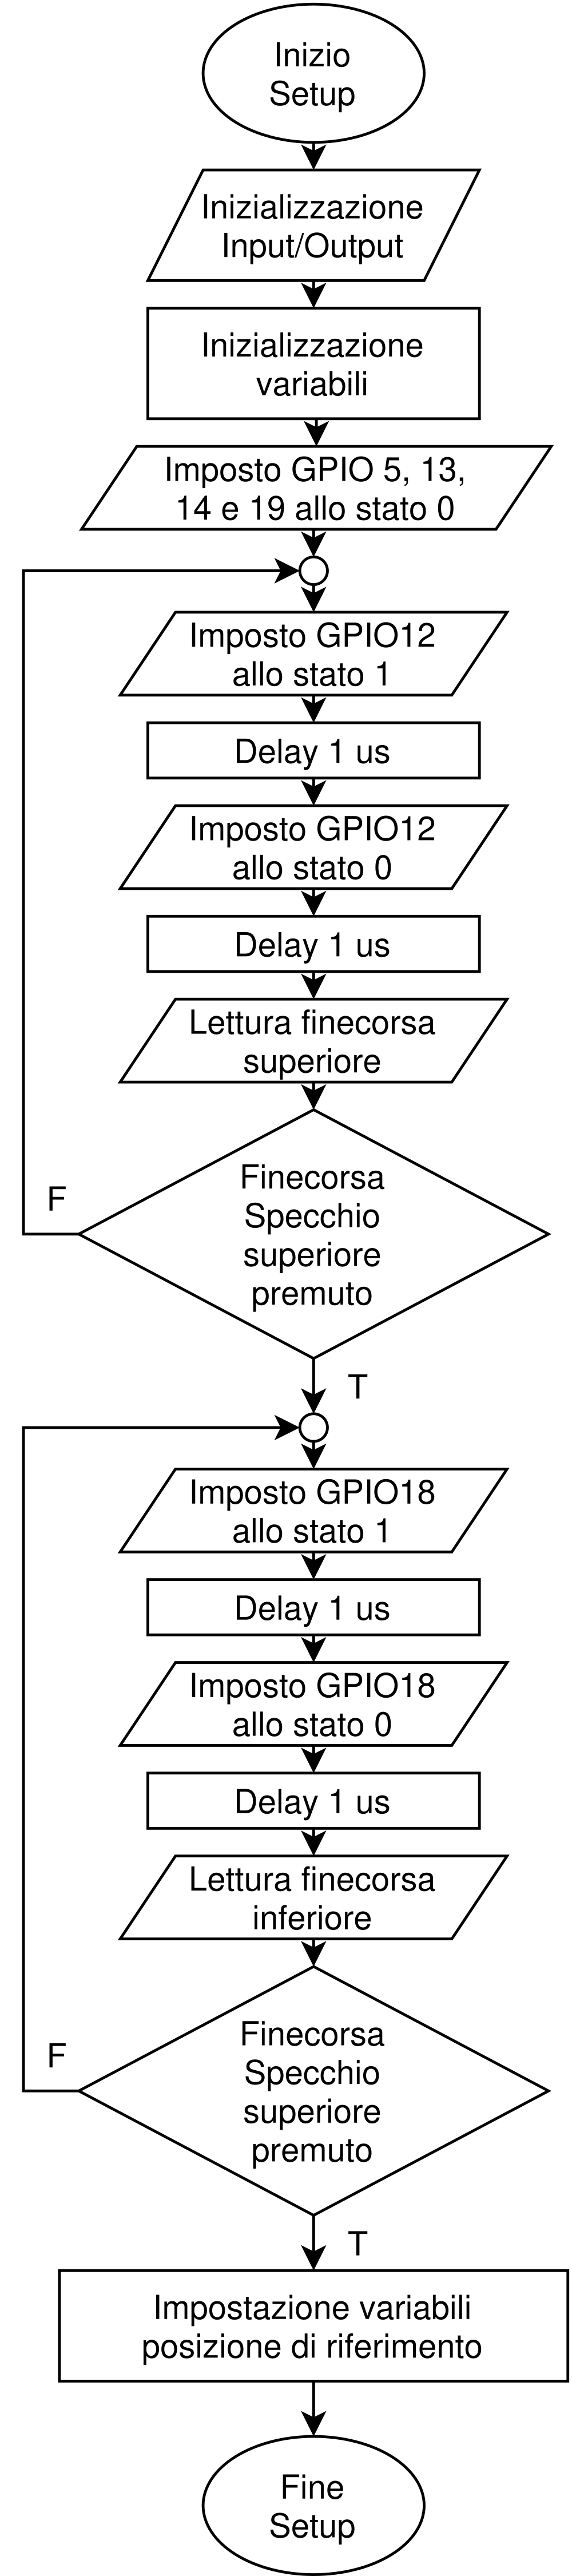
\includegraphics[height=\textheight-150pt]{Draws/Flowchart/Setup.png}
                \label{setup_flowchart}
            \end{center}
        
        \subsubsection{Loop}
            \begin{center}
                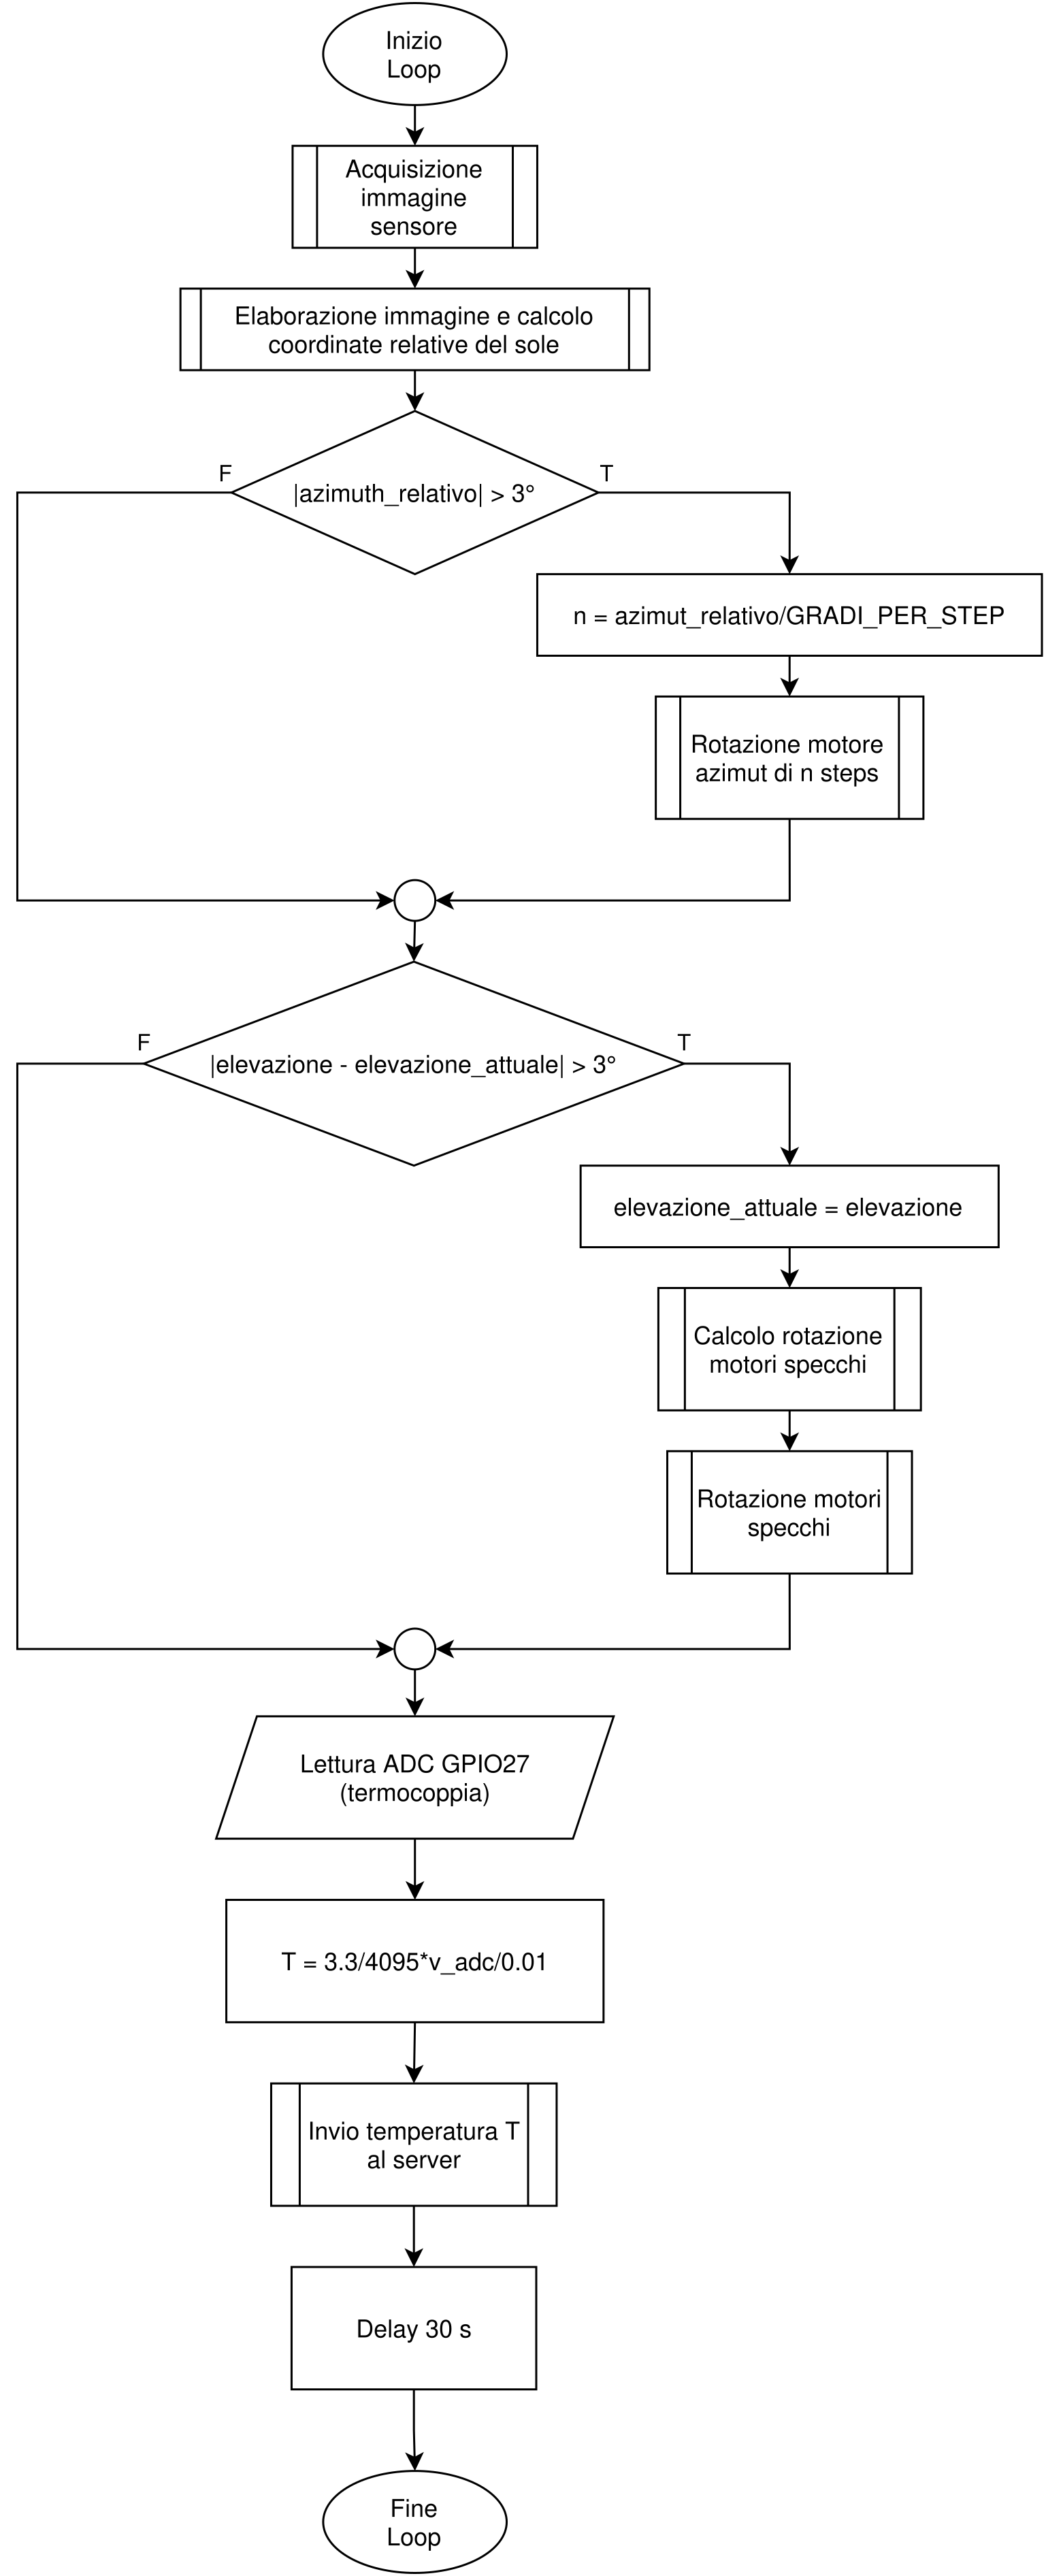
\includegraphics[height=\textheight-40pt]{Draws/Flowchart/Loop.png}
            \end{center}
        
    \subsection{Analisi funzioni principali}
        \subsubsection{Controllo accelerazione motori}
        Il driver A4988 permette il controllo della rotazione dei motori mediante un segnale di direzione e uno di step: ogni fronte di salita del segnale di step comporta un incremento della posizione del motore nella direzione selezionata dal segnale di direzione, tale incremento dipende, oltre che dalle caratteristiche strutturali del motore in questione, dal rapporto di micro-stepping.\\
        La rotazione è quindi composta da brevi scatti successivi, maggiore è il numero di microstep per step e maggiore sarà la fluidità del movimento.\\
        Un semplice controllo ON-OFF, con accesione dei motori direttamente ad una velocità definita e costante, provoca elevate accelerazioni che portano ad una maggiore usura dei componenti meccanici, oltre che possibili oscillazioni attorno alla posizione desiderata, per questo motivo risulta opportuno variare la velocità grazualmente per ottenere accelerazioni e decelerazioni costanti.\\
        
        \begin{figure}[h]
        \centering
            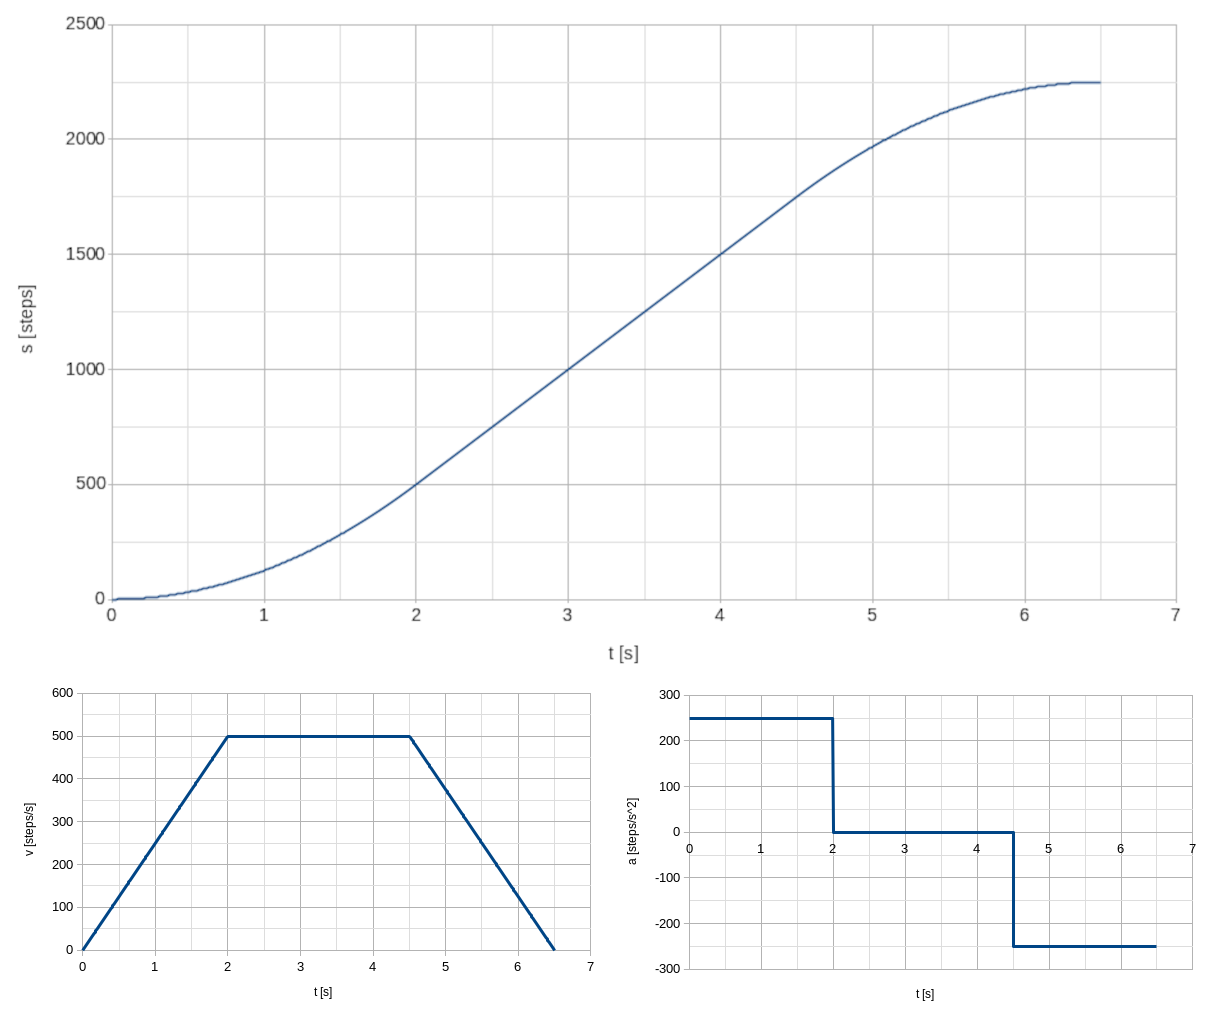
\includegraphics[width=\textwidth-25pt]{Draws/Motors_s-v-a_block.png}
            \caption{Andamento steps nel tempo}
            \label{Steps_velocity_acceleration_in_time}
        \end{figure}
        
        
        L'andamento nel tempo mostrato in figura \ref{Steps_velocity_acceleration_in_time} può essere suddiviso in 3 fasi: una iniziale di accelerazione (ad accelerazione costante), un'eventuale fase centrale a velocità costante ed una finale di decelerazione (con accelerazione costante e opposta a quella iniziale).\\
        
        Ricordando le equazioni del moto uniformemente accelerato, si ha:
        \begin{equation}
            s(t) = s_0 + v_0 \cdot t + \frac{1}{2} \cdot a \cdot t^2
        \end{equation}
        \begin{equation}
            v(t) = v_0 + a \cdot t
        \end{equation}       
        

        \vspace{0.1cm}

        Una possibile implementazione per il microcontrollore in considerazione può essere la seguente\footnote{Questa funzione fa parte del programma completo nel suo complesso, per cui vi sono riferimenti a variabili globali e costanti non definite all'interno di questa funzione.}.
        
        
        \begin{changemargin}{-2cm}{-2cm}
        \begin{lstlisting}[label={list:motor_speed_control}, style=Arduino, caption=Controllo velocità motori, basicstyle=\scriptsize]
long move_stepper (long n_steps, float speed, float acceleration, int dir_pin, int step_pin, int enable_pin, int endstop) {    // speed in steps/s, acceleration in steps/s^2
  if (n_steps < 0) {
    digitalWrite(dir_pin, HIGH);
  } else {
    digitalWrite(dir_pin, LOW);
  }

  unsigned long t_offset = micros();
  unsigned long t;
  unsigned long acceleration_limit_steps = 0.5 * speed * speed / acceleration + 0.5;
  bool acceleration_phase = true;
  bool constant_phase = false;
  bool deceleration_phase = false;
  bool condition;

  if (acceleration_limit_steps > abs(n_steps) / 2) {
    acceleration_limit_steps = abs(n_steps) / 2;
    speed = sqrt(2 * acceleration_limit_steps * acceleration);
  }

  digitalWrite(enable_pin, LOW);
  for (long microsteps = 0; microsteps < abs(n_steps)*MICROSTEPPING_RATIO; microsteps++){
    do {
      t = micros();
      if (constant_phase) {
        condition = ((microsteps / MICROSTEPPING_RATIO - acceleration_limit_steps) * 1000 > speed * (t - t_offset) / 1000.0);
      } else if (acceleration_phase) {
        condition = (microsteps * 1000000.0 / MICROSTEPPING_RATIO > 0.5 * acceleration * ((t - t_offset) / 1000.0) * ((t - t_offset) / 1000.0));
      } else if (deceleration_phase) {
        condition = (((microsteps / MICROSTEPPING_RATIO - (abs(n_steps) - acceleration_limit_steps)) * 1000000) > (speed * (t - t_offset) - 0.5 * acceleration * ((t - t_offset) / 1000.0) * ((t - t_offset) / 1000.0)));
        if (condition) {
          if (t - t_offset > speed / acceleration * 1000000) {
            condition = false;
          }
        }
      }
    } while (condition);
    
    if (!digitalRead(endstop)) {
      digitalWrite(step_pin, HIGH);
      delayMicroseconds(2);      // Pulse must be at least 1us (from A4988 datasheet)
      digitalWrite(step_pin, LOW);
      delayMicroseconds(1);      // Pulse must be at least 1us (from A4988 datasheet)
      if (constant_phase) {
        if (microsteps / MICROSTEPPING_RATIO >= abs(n_steps) - acceleration_limit_steps) {
          constant_phase = false;
          deceleration_phase = true;
          t_offset = micros();
        }
      } else if (acceleration_phase) {
        if (microsteps / MICROSTEPPING_RATIO >= acceleration_limit_steps) {
          acceleration_phase = false;
          constant_phase = true;
          t_offset = micros();
        }
      }
    } else {
      if (disable_motor) {
        digitalWrite(enable_pin, HIGH);
      }
      return microsteps;
    }
  }
  if (disable_motor) {
    digitalWrite(enable_pin, HIGH);
  }
}       \end{lstlisting}
        \end{changemargin}
        
        \newpage
        \subsubsection{Protocollo sensore ottico}\label{adns2610_protocol}
        
        Il sensore ADNS2610 utilizza un protocollo digitale sincrono che permette la lettura e scrittura di registri interni con diverse funzioni. Per l'applicazione in questione è rilevante il registro 0x08, che alla $i$-esima lettura dell'ultima scrittura in questo registro fornisce un byte riguardante l'$i$-esimo pixel (ripartendo dal primo quando si raggiunge l'ultimo pixel): il bit più significativo  indica se il pixel è o meno il primo dell'immagine; il bit successivo è posto a 1 se e solo se il dato è corretto e può essere letto; i restanti 6 bit rappresentano la luminosità del pixel in questione.
        
        Ogni comunicazione è iniziata dal master, che controlla il clock, e trasmette un bit che indica se intende scrivere o leggere un registro, seguito da 7 bit indicanti l'indirizzo del registro stesso (MSB-first).
        
        \begin{figure}[h]
        \centering
            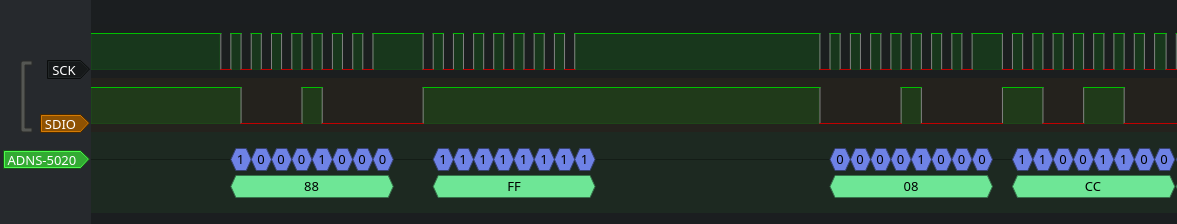
\includegraphics[width=\textwidth]{Draws/Logic_analyzer_ADNS2610.png}
            \caption{Diagramma temporale protocollo comunicazione}
        \end{figure}
        
        Nel diagramma precedente si osserva chiaramente una prima comunicazione che scrive nel registro 0x08 (per resettare lo stato interno e leggere successivamente il primo pixel) seguita da una lettura dello stesso registro che ritorna la luminosità del primo pixel.
      
        \vspace{2cm}
        Un possibile esempio di implementazione può essere il seguente\footnote{Come nell'esempio precedente vi sono variabili globali non definite, in particolare la variabile "matrix" conterrà la matrice rappresentante l'immagine acquisita}.
        
        \begin{changemargin}{-2cm}{-2cm}
        \begin{lstlisting}[label={list:protocol_implementation}, style=Arduino, caption=Lettura immagine da sensore, basicstyle=\scriptsize]
int i = 0;
while (i < 18 * 18) {
  delayMicroseconds(1);
  uint8_t data = read(0x08);
  if (data & 0b01000000) {
    matrix[i/18][i%18] = data;
    i++;
  }
}


void write(uint8_t register_addr, uint8_t data) {
  register_addr |= 0b10000000;                  // Set MSB to 1
  write_byte(register_addr);
  delayMicroseconds(200);
  write_byte(data);
  delayMicroseconds(200);
}

uint8_t read(uint8_t register_addr) {
  register_addr &= 0b01111111;                  // Set MSB to 0
  write_byte(register_addr);
  pinMode(SDIO, INPUT);                         // High-Z mode
  delayMicroseconds(100);                       // T_hold >= 100us from specifications

  uint8_t read_data = 0;
  for (int8_t i = 7; i >= 0; i--) {
    digitalWrite(SCK, LOW);                     // Start clock signal
    delayMicroseconds(50);                      // Same as mouse application
    digitalWrite(SCK, HIGH);                    // Data must be read on transition from 0 to 1
    read_data += digitalRead(SDIO) << i;        // Data line must be read here
    delayMicroseconds(50);                      // Same as mouse application
  }
  return read_data;
}


void write_byte (uint8_t byte_val) {
  pinMode(SDIO, OUTPUT);

  for (int8_t i = 7; i >= 0; i--) {
    digitalWrite(SCK, LOW);                     // Start clock signal
    digitalWrite(SDIO, byte_val & (1 << i));    // Data line must be set here
    delayMicroseconds(50);                      // Same as mouse application
    digitalWrite(SCK, HIGH);                    // A2610 latchs data on transition from 0 to 1
    delayMicroseconds(50);                      // Same as mouse application
  }
}       \end{lstlisting}
        \end{changemargin}
        
        \newpage
        \subsubsection{Edge detection}\label{edge_detection}
        Per determinare i contorni di una figura in un'immagine i sistemi di visione, solitamente, valutano la differenza di colore, o luminosità, tra pixel successivi, in quanto maggiore è tale differenza e più è netto il contorno composto da quei pixel.
        
        Matematicamente possiamo definire per una matrice $I$ $m \times n$, una seconda matrice $G$ di dimensioni $(m-2) \times (n-2)$ tale che:
        \begin{equation}\label{edge_detection_equation}
        \begin{split}
            G_{y, x} = \sqrt{\left(I_{y, x} - I_{y, x+2}\right)^2 + \left( I_{y, x} - I_{y+2, x} \right)^2} \\
            \forall \quad 1 \leq x \leq n-2 \qquad
            1 \leq y \leq m-2
        \end{split}
        \end{equation} 
        
        Che, nel caso in cui $I$ rappresenti la luminosità dei pixel dell'immagine, equivale al modulo del vettore composto da due componenti ortogonali costituite, rispettivamente, dalla differenza di luminosità tra il pixel precedente-successivo (E-C) e superiore-inferiore (B-D) a quello considerato (A in figura).
        
        \begin{figure}[h]
        \centering
            
\includegraphics[width=130pt]{Draws/Edge_detection_pixel_label.png}
            \caption{Disposizione pixel}
        \end{figure}
        
        L'implementazione \footnote{Come del codice \ref{list:protocol_implementation} la variabile globale "matrix" rappresenta i pixel dell'immagine acquisita, mentre "gradient\_modules" conterrà il risultato del'operazione} di questa operazione è molto semplice, in quanto consiste solamente nel ciclare tra gli indici della matrice e applicare la formula (\ref{edge_detection_equation}).
        \begin{changemargin}{-2cm}{-2cm}
        \begin{lstlisting}[label={list:edge_detection_code}, style=Arduino, caption=Calcolo matrice edge-detection, basicstyle=\scriptsize]
void calculate_gradient_matrix () {
  for (int8_t y = 0; y < 16; y++) {
    for (int8_t x = 0; x < 16; x++) {
      gradient_modules[y][x] = sqrt(pow(matrix[y + 2][x + 1] - matrix[y][x + 1], 2) + pow(matrix[y + 1][x + 2] - matrix[y + 1][x], 2)) + 0.5;
    }
  }
}       \end{lstlisting}
        \end{changemargin}
        
        
        Nella seguente immagine si può osservare l'applicazione tale algoritmo ad una immagine acquisita dal sensore.
        
        \begin{figure}[h]
        \centering
            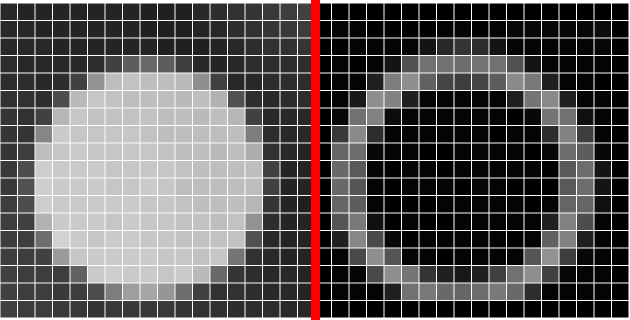
\includegraphics[width=300pt]{Draws/default_image-gradient.png}
            \caption{Edge-detection su immagine acquisita dal sensore}
            \label{edge-detection_image_comparison}
        \end{figure}
        
        
        \subsubsection{Discesa del gradiente}\label{gradient_descent}
        Per ottenere il centro dell'immagine del sole, che approssimiamo ad un cerchio, è sufficiente trovare la circonferenza che meglio approssima il contorno esterno del cerchio, definito dai punti in cui si ha una differenza più netta tra pixels successivi. \\
        A tal fine si deve minimizzare la distanza geometrica tra la circonferenza e i punti con magiore modulo del vettore trattato nella sezione \ref{edge_detection}; tale distanza è schematizzata nella seguente figura con il tratto $ e $.

        \begin{figure}[h]
        \centering
            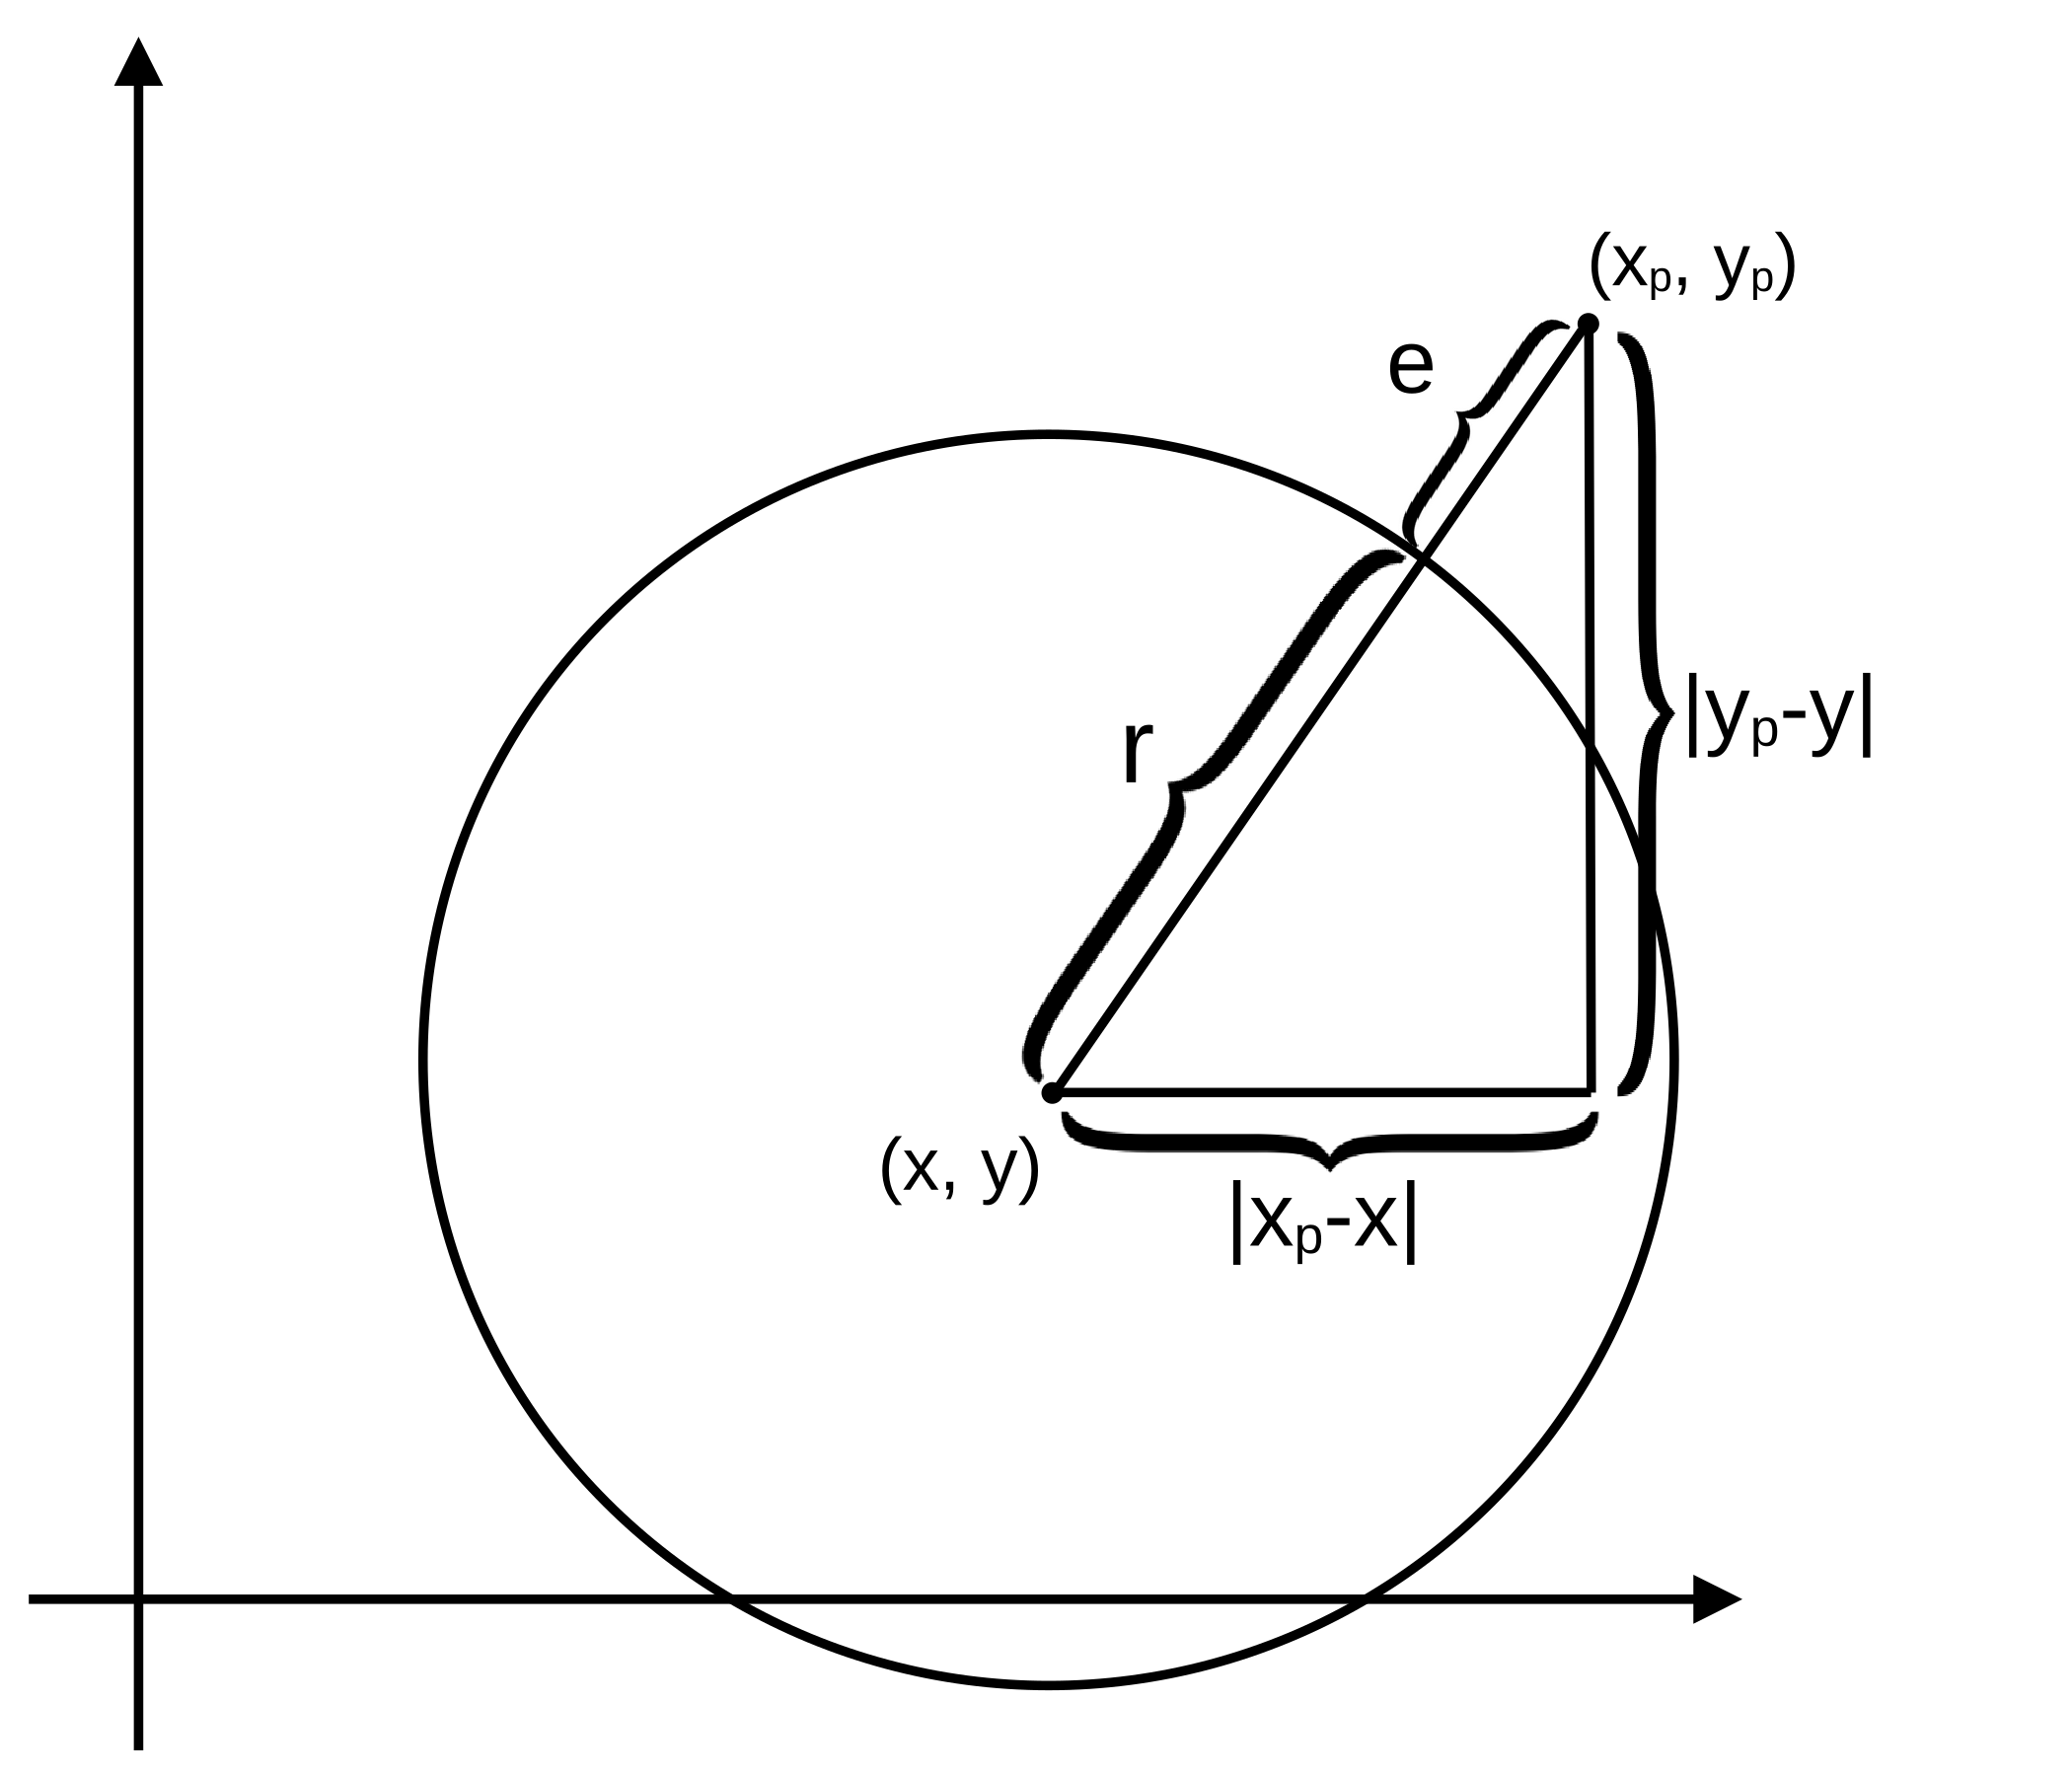
\includegraphics[width=260pt]{Draws/Discesa_del_gradiente_cerchio-punto.png}
            \caption{Distanza punto - circonferenza}
        \end{figure}
        
        
        Applicando il teorema di pitagora, per differenza, si ottiene che la distanza $ e $ è definita in funzione delle coordinate del centro e del punto in questione, secondo la relazione
        \begin{equation}
             e = \left| \sqrt{(x_p-x)^2 + (y_p-y)^2} -r \right|
        \end{equation}
        
        
        Possiamo quindi definire la seguente funzione\footnote{Per semplicità di seguito si assume che per una matrice $m \times n$ gli indici degli elementi assumano valori partendo da 0, ad esempio l'elemento della prima riga e colonna sarà $G_{0,0}$, mentre l'elemento dell'ultima riga e colonna sarà $G_{m-1, n-1}$. Questo perché nella maggior parte dei linguaggi di programmazione l'indice del primo elemento di un array è proprio 0.}
        \begin{equation}
            f(x, y, r) = \sum_{y_p = 0}^{15} \sum_{x_p = 0}^{15} \left[ G_{y_p, x_p} \cdot \left| \sqrt{(x_p-x)^2 + (y_p-y)^2} -r \right| \right] 
        \end{equation}
        
        
        in cui la matrice $ G_{y_p, x_p} $ rappresenta il modulo del gradiente dell'immagine del punto $ (x_p, y_p) $, come trattato nella sezione \ref{edge_detection}, ed è quindi un coefficiente reale. Tale sommatoria risulta quindi una somma ponderata delle distanze tra la circonferenza in considerazione e tutti i punti della matrice discussa alla sezione precedente. Il modulo del gradiente sarà maggiore per i punti sul contorno dell'immagine del sole, che quindi avranno un peso maggiore rispetto agli altri.\\
        
        Il problema risulta quindi equivalente alla ricerca del minimo di tale funzione, per questo scopo può essere utile considerare il caso più semplice di una funzione ad una sola variabile.
        
        \begin{figure}[h]
        \centering
            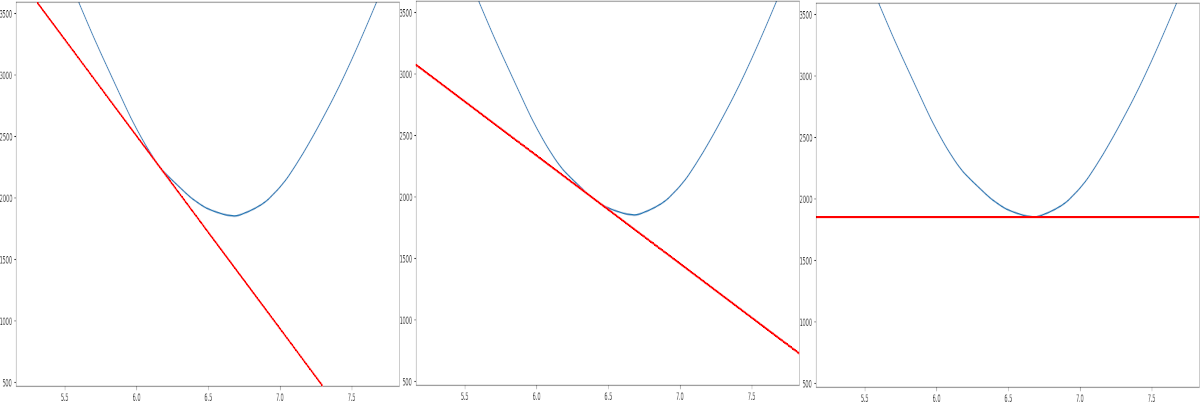
\includegraphics[width=\textwidth]{Draws/matplotlib_draws/2d_descent_block.png}
            \caption{Ricerca minimo - 2D}
            \label{2d_min_search}
        \end{figure}
        
        Nell'immagine \ref{2d_min_search} si osserva la funzione rappresentativa dell'errore al variare della variabile $r$, fissati $x$ e $y$, nel caso dell'immagine rappresentata in figura \ref{edge-detection_image_comparison}, mentre la retta rossa indica la tangente alla curva. Si osservi che, partendo da un punto iniziale sulla curva, è possibile individuare un minimo locale variando l'ascissa corrente di un valore $-k \cdot f'(r)$, con $k$ scelto opportunamente (e positivo), e iterando questo procedimento fino ad ottenere l'approssimazione desiderata.\\
        
        È possibile applicare lo stesso algoritmo per una funzione in due variabili, rappresentabile come una superficie in uno spazio tridimensionale.
        
        \begin{figure}[h]
        \centering
            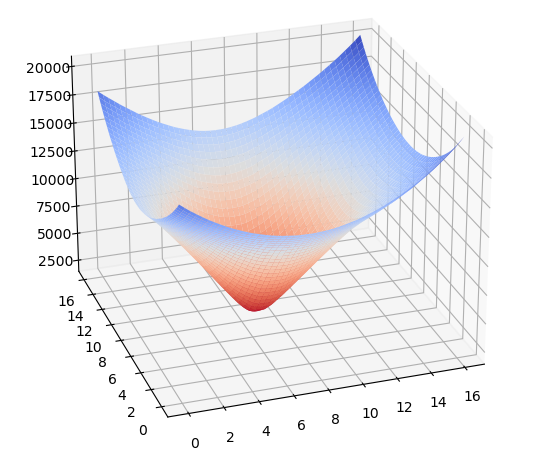
\includegraphics[width=\textwidth-50pt]{Draws/matplotlib_draws/3d_descent_base_cut.png}
            \caption{Ricerca minimo - 3D}
            \label{3d_min_search}
        \end{figure}
        
        In cui il minimo può essere trovato nuovamente iterando più volte un procedimento analogo al precedente, considerando entrambe le derivate parziali della funzione.\\
        
        
        \vspace{1cm}
        Nella situazione in questione i le variabili sono tre ($x$, $y$ e $r$), per cui la funzione può essere rappresentata geometricamente in uno spazio a 4 dimensioni, che associa ad ogni punto dello spazio tridimensionale un valore proporzionale all'errore, per questo motivo possiamo rappresentare il valore assunto dalla funzione mediante una scala cromatica e visualizzarne l'andamento.
        
        \begin{figure}[h]
        \centering
            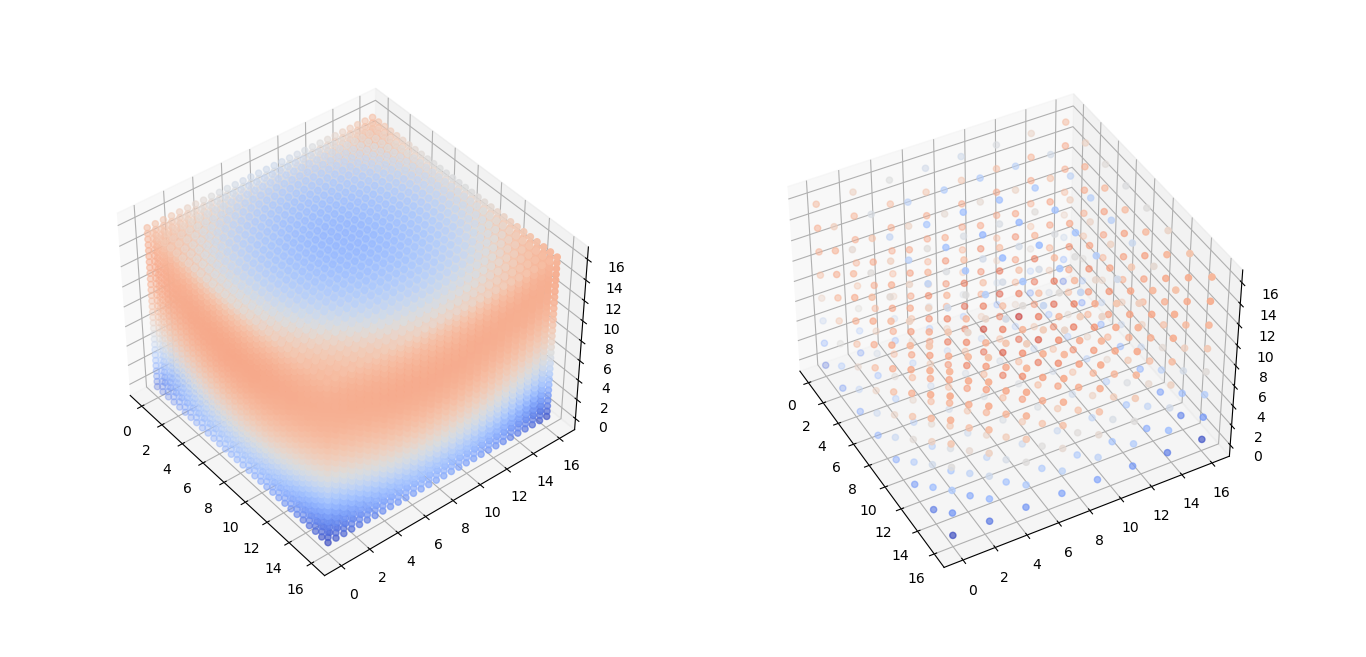
\includegraphics[width=\textwidth]{Draws/matplotlib_draws/4d_descent_volume_block.png}
            \caption{Ricerca minimo - 4D}
            \label{4d_min_search}
        \end{figure}
        
        \vspace{1cm}
        Calcoliamo quindi le derivate parziali di $ f(x, y, r) $ rispetto alle tre variabili (non essendovi uno standard univoco, di seguito si è scelto di utilizzare la notazione di Leibniz per indicare derivate e derivate parziali)
        
        \begin {equation}
            \frac{\partial f}{\partial x} = \sum_{y_p = 0}^{15} \sum_{x_p = 0}^{15} \left[ G_{y_p, x_p} \cdot sgn \left( \sqrt{(x_p-x)^2 + (y_p-y)^2} - r \right) \cdot \frac{x - x_p}{\sqrt{(x_p - x)^2 + (y_p - y)^2}} \right] 
        \end {equation}
        \begin {equation}
            \frac{\partial f}{\partial y} = \sum_{y_p = 0}^{15} \sum_{x_p = 0}^{15} \left[ G_{y_p, x_p} \cdot sgn \left( \sqrt{(x_p-x)^2 + (y_p-y)^2} - r \right) \cdot \frac{y - y_p}{\sqrt{(x_p - x)^2 + (y_p - y)^2}} \right] 
        \end {equation}
        \begin {equation}
            \frac{\partial f}{\partial r} = \sum_{y_p = 0}^{15} \sum_{x_p = 0}^{15} \left[ - G_{y_p, x_p} \cdot sgn \left( \sqrt{(x_p-x)^2 + (y_p-y)^2} - r \right) \right] 
        \end {equation}
        
        
        con $ sgn(x)$ definita a tratti nel dominio $(- \infty ; 0) \cup (0; +\infty) $ :
        
        \begin {equation}
            sgn(x) = 
                \begin{cases}
                  -1 & \text{se x < 0} \\
                  1 & \text{se x > 0}
                \end{cases}
        \end {equation}
        
        
        Definiamo il gradiente calcolato in un punto $(x_0, y_0, r_0)$ di una funzione $f(x)$ come la seguente funzione vettoriale
        
        \begin{equation}
            \nabla f (x_0, y_0, r_0) = \left( \frac{\partial f}{\partial x} \bigg\rvert_{x = x_0}, \frac{\partial f}{\partial y} \bigg\rvert_{y = y_0}, \frac{\partial f}{\partial r} \bigg\rvert_{r = r_0} \right)
        \end{equation}
        
        \vspace{1cm}
        Ad ogni iterazione dell'algoritmo si otterrà uno spostamento proporzionale a tale vettore, per cui alla $i$-esima ripetizione si avrà:
         
        \begin{equation}
            (x_i, y_i, r_i) = (x_{i-1}, y_{i-1}, r_{i-1}) - k \cdot \nabla f (x_{i-1}, y_{i-1}, r_{i-1}) \qquad con \quad k > 0
        \end{equation}
        
        Essendo un algoritmo euristico esso non garantisce di trovare con esattezza un punto di minimo, ma una sua approssimazione (che per il caso in esame è più che sufficiente); inoltre il punto trovato è un minimo locale, ma non è garantito che sia un minimo assoluto, come mostrato nell'immagine \ref{double_min}, per questo può essere opportuno ripetere il procedimento scegliendo diversi punti di partenza, oppure approssimare il centro con altri metodi e utilizzare il valore trovato come punto iniziale (quest'ultimo metodo risulta particolarmente efficace e può essere realizzato con una media ponderata delle coordinate dei pixel dell'immagine, pesati sulla loro luminosità).
        
        \begin{figure}[h]
        \centering
            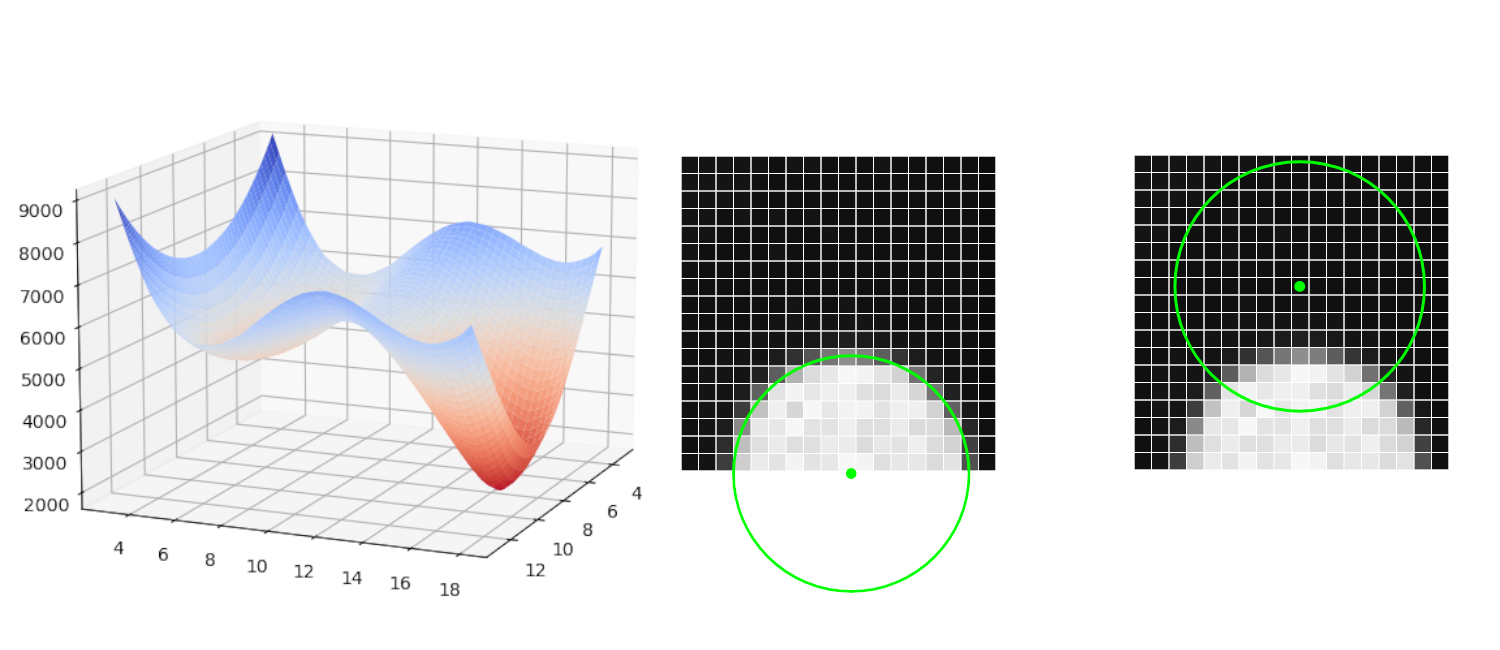
\includegraphics[width=\textwidth]{Draws/matplotlib_draws/double_min_block.png}
            \caption{Minimo locale e minimo assoluto}
            \label{double_min}
        \end{figure}
        
        Il minimo locale e il minimo assoluto corrispondono rispettivemente alla circonferenza mostrata nell'immagine di destra e di sinistra.\\

        \newpage
        Un possibile esempio di implementazione è il seguente\footnote{Come per le porzioni di codice precedenti, esso fa riferimento a costanti e variabili globali non riportate in questo documento.}.
        
        \begin{changemargin}{-2cm}{-2cm}
        \begin{lstlisting}[label={list:gradient_descent}, style=Arduino, caption=Ricerca minimi - discesa del gradiente, basicstyle=\scriptsize]
void gradient_descent (float x, float y, float r, uint16_t iterations) {
  for (uint16_t recurse_n = 0; recurse_n < iterations; recurse_n++) {
    float dx = 0.0, dy = 0.0, dr = 0.0;
    for (uint8_t y_p = 0; y_p < 16; y_p++) {
      for (uint8_t x_p = 0; x_p < 16; x_p++) {
        if (gradient_modules[y_p][x_p] > GRADIENT_THRESHOLD) {
          float x_diff = x_p - x;
          float y_diff = y_p - y;
          float x_diff_2 = pow(x_diff, 2);
          float y_diff_2 = pow(y_diff, 2);
          if ((x_diff_2 + y_diff_2) == 0) {
            continue;
          }
          dx -= (gradient_modules[y_p][x_p] - GRADIENT_THRESHOLD) * SGN(sqrt(x_diff_2 + y_diff_2) - r) * x_diff / sqrt(x_diff_2 + y_diff_2);
          dy -= (gradient_modules[y_p][x_p] - GRADIENT_THRESHOLD) * SGN(sqrt(x_diff_2 + y_diff_2) - r) * y_diff / sqrt(x_diff_2 + y_diff_2);
          dr -= (gradient_modules[y_p][x_p] - GRADIENT_THRESHOLD) * SGN(sqrt(x_diff_2 + y_diff_2) - r);
        }
      }
    }

    x -= dx * K;
    y -= dy * K;
    r -= dr * K;
    progressive_approximations[recurse_n * 3] = x - 7.5;
    progressive_approximations[recurse_n * 3 + 1] = y - 7.5;
    progressive_approximations[recurse_n * 3 + 2] = r;
  }
}       \end{lstlisting}
        \end{changemargin}

    \newpage
    \section{Conclusioni e considerazioni}
    Dal grafico mostrato in figura \ref{accuracy_test} si può osservare che il metodo in esame fornisce risultati sufficientemente accurati e gli errori registrati possono derivare da errori di misura oltre che dalle effettive imprecisioni del sistema di acquisizione e di elaborazione dell'immagine.
    
    \begin{figure}[h]
    \centering
        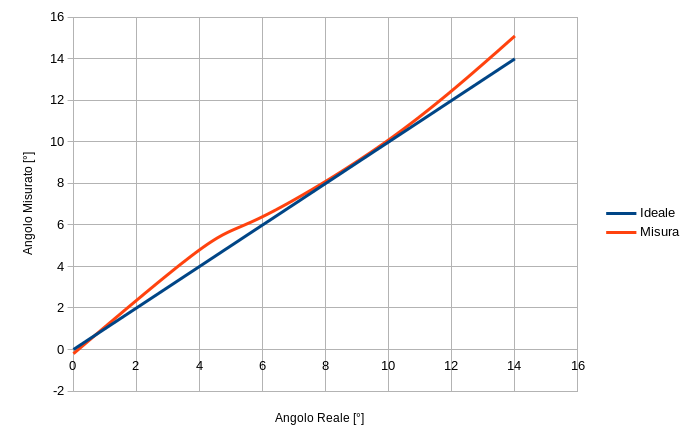
\includegraphics[width=\textwidth-50pt]{Draws/Accuracy_test.png}
        \caption{Prova di accuratezza}
        \label{accuracy_test}
    \end{figure}
     
    Inoltre la prova è stata effettuata utilizzando il foro normalmente in dotazione con il sensore, che limita l'angolo di campo a circa 40° (mantenendo risultati accettabili), tuttavia di può ovviare a questo problema come discusso nella sezione \ref{optical_sensor} oppure con l'aggiunta di un sistema ottico di lenti ed eventualemente utilizzando un sensore con una maggiore risoluzione.
    
    \vspace{1cm}
    L'algoritmo per minimizzare il valore della funzione, trattato nella sezione \ref{gradient_descent}, è tipicamente utilizzato in algoritmi di intelligenza artificiale, in particolare machine learning, per la sua flessibilità, infatti la funzione da minimizzare può rappresentare diverse grandezze a seconda della situazione in esame e i parametri possono essere perfezionati all'aumentare dei campioni disponibili, senza dover modificare l'algoritmo in sé.
    
    \newpage
    La relizzazione pratica e concreta di questo progetto richiede diversi processi e apparecchiature. In particolare la produzione dei circuiti stampati per un'installazione stabile e professionale richiede l'utilizzo di macchine a controllo numerico, come ad esempio fresatrice CNC, per la creazione di vie, fori e piste; inoltre per la rimozione del rame in eccesso dalla lastra ramata, durante la fase di creazione delle piste, vengono usate sostanze chimiche particolarmente corrosive e tossiche se ingerite, come il cloruro ferrico. Quindi il tema della sicurezza e l'utilizzo degli appositi DPI (Dispositivi di Protezione Individuale) sono elementi essenziali per la tutela dei lavoratori che operano nella produzione di questi prodotti. Inoltre, anche il dispositivo durante il funzionamento avrà dei rischi dovuti alle alte temperature che si possono raggiungere al suo interno (rischio di ustioni) e alle parti meccaniche in movimento (rischio di schiacciamento).
    
    \vfill
    \let\thefootnote\relax\footnotetext{
        \begin{center}
            Documento realizzato in \LaTeX.
        \end{center}
    }
\end{document}

